\documentclass[12pt]{article}

% graphicx package, useful for including eps and pdf graphics
\usepackage{graphicx}
\DeclareGraphicsExtensions{.png,.png,.jpg}

% basic packages
\usepackage{color}
\usepackage{parskip}
\usepackage{float}
\usepackage{microtype}
\usepackage{url}
\usepackage{hyperref}
\usepackage{booktabs}
\usepackage{makecell}

% text layout
\usepackage{geometry}
\geometry{textwidth=17cm} % 15.25cm for single-space, 16.25cm for double-space
\geometry{textheight=22.5cm} % 22cm for single-space, 22.5cm for double-space

% helps to keep figures from being orphaned on a page by themselves
\renewcommand{\topfraction}{0.85}
\renewcommand{\textfraction}{0.1}

% bold the 'Figure #' in the caption and separate it with a period
% Captions will be left justified
\usepackage[labelfont=bf,labelsep=period,font=small]{caption}

% cite package, to clean up citations in the main text. Do not remove.
\usepackage{cite}

\usepackage{authblk}
\renewcommand\Authands{ \& }
\renewcommand\Authfont{\normalsize \bf}
\renewcommand\Affilfont{\small \normalfont}
\makeatletter
\renewcommand\AB@affilsepx{, \protect\Affilfont}
\makeatother

% comments
\usepackage{ulem}
\definecolor{purple}{rgb}{0.459,0.109,0.538}
\def\tbc#1{\textcolor{purple}{[#1]}}
% \def\rnc#1{\textcolor{blue}{[#1]}}
% \def\jhc#1{\textcolor{green}{[#1]}}

\title{Antigenic phenotypes and phylogenetic metrics improve forecasts of seasonal influenza A/H3N2 evolution}
%\title{Improved forecasts of seasonal influenza A/H3N2 evolution}
%\title{Integrative forecasting of seasonal influenza A/H3N2 by genotype and phenotype}
%\title{Experimentally informed forecasts of seasonal influenza A/H3N2}
%\title{Long-term forecasts of seasonal influenza reveal historical contingency of fitness metrics}

\author[1,2]{John Huddleston}
\author[3]{Richard A.\ Neher}
\author[1]{Trevor Bedford}

\affil[1]{Vaccine and Infectious Disease Division, Fred Hutchinson Cancer Research Center, Seattle, WA, USA}
\affil[2]{Moleculary and Cell Biology, University of Washington, Seattle, WA, USA}
\affil[3]{Biozentrum, University of Basel, Basel, Switzerland}

\date{}

\begin{document}

\begin{abstract}
Seasonal influenza virus A/H3N2 is a major cause of illness and death globally.
While vaccination is the most effective way to prevent infection, rapid accumulation of mutations in the surface protein hemagglutinin (HA) allows viruses to escape previous adaptive immunity due to vaccination or natural infection.
This antigenic drift requires vaccines to be updated regularly.
Due to a nearly one-year lag between the selection of vaccine strains and deployment of the vaccine to the public, effective vaccine strain selection requires predictions about future influenza populations.
Historically, experts predicted successful future viruses through manual inspection of hemagglutination inhibition (HI) assays, an experimental measure of antigenic drift.
Modern strain selection is increasingly informed by modeling of influenza fitness using HA sequences to estimate antigenic drift, mutational load, and recent population growth.
The models rely entirely on genotypic information without accounting for the gold standard phenotypic measures of antigenic drift provided by HI assays.
We developed a novel open source forecasting framework based on these original fitness models that explicitly integrates genotypic and phenotypic measures of antigenic drift as well as modern experimental measurements of mutational load from deep mutational scanning (DMS) experiments.
In contrast with previous work, our models minimize the distance between observed and estimated future populations using the Earth Mover's Distance metric instead of minimizing errors in frequencies of phylogenetic clades.
We show that this integrated approach to forecasting can accurately estimate the sequence compositions of simulated and natural populations.
These forecasts capture dynamics of influenza clades and enable the identification of optimal individual strains for vaccine composition.
Using this framework and a modern machine learning approach to model testing, we found that phenotypic measures of antigenic drift were more consistently predictive of future influenza populations than sequence-only measures while the opposite was true for measures of mutational load.
Importantly, the combination of antigenic drift and mutational load was the most predictive of future success.
We provide real-time forecasts of seasonal influenza A/H3N2 populations based on our combined model of antigenic drift and mutational load as part of Nextstrain.
As our open source framework allows definition of fitness metrics per sample using tidy data frames and does not require phylogenetic clades for forecasts, we hope it paves the way for future forecasting efforts with pathogens that cannot be readily analyzed by standard phylogenetic methods including recombinant viruses, bacteria, and fungi.

\end{abstract}

\maketitle


\section*{Introduction}

Seasonal influenza virus infects 5--15\% of the global population every year causing an estimated 250,000 to 500,000 deaths annually \cite{flufactsheet}.
Vaccination remains the most effective public health response available.
However, frequent viral mutation results in viruses that escape previously acquired human immunity.
The World Health Organization (WHO) selects vaccine viruses to match circulating viruses, but because the process of vaccine development and distribution requires several months to complete, accurate vaccine strain selection requires a prediction of which viruses will predominate approximately one year after vaccine viruses are selected.
Current vaccine predictions favor viruses that are distinct from prior vaccine viruses in the hemagglutinin (HA) protein, which acts as the primary target of human immunity.
The hemagglutination inhibition (HI) assay \cite{hirst1943studies} is used to measure the degree of cross-reactivity between pairs of circulating viruses.
HI assays are fundamental for vaccine strain selection, but they are laborious and low-throughput compared to genome sequencing \cite{Wood:2012ii}.
As a result, researchers have developed computational methods to predict influenza fitness from sequence data alone \cite{Luksza:2014hj,Steinbruck:2014kq,Neher:2014eu}.

Despite the promise of these sequence-only models, they explicitly omit experimental measurements of antigenic or functional phenotypes.
Recent developments in computational methods and influenza virology have made it feasible to integrate these important metrics of influenza fitness into a single predictive model.
For example, phenotypic measurements of antigenic drift are now accessible through phylogenetic models \cite{Neher:2016hy} and functional phenotypes for HA are available from deep mutational scanning experiments \cite{Lee2018}.
We describe an approach to integrate previously disparate sequence-only models of influenza evolution with high-quality experimental measurements of antigenic drift and functional constraint.

The influenza community has long recognized the importance of incorporating HI phenotypes and other experimental measurements of viral phenotypes with existing forecasting methods into an extensible, open source framework that can be used by professional virologists in their vaccine design process \cite{Gandon:2016gz,Morris:2017ea,Lassig:2017hr}.
Although several distinct efforts have made progress in using HI phenotypes to evaluate the evolution of seasonal influenza \cite{Steinbruck:2014kq,Neher:2016hy}, these methods stop short of developing a complete forecasting framework wherein the evolutionary contribution of HI phenotypes can be compared and contrasted with new and existing fitness metrics.
Here, we provide the first such open source long-term forecasting framework for seasonal influenza.
With this framework, we show that HI phenotypes enable more accurate long-term forecasts of A/H3N2 populations compared to previous metrics based on epitope mutations alone.
However, we also find that phylogenetic fitness metrics based on recent growth of circulating clades consistently outperform any combination of genotypic or phenotypic metrics, suggesting that existing mechanistic models of seasonal influenza evolution are missing critical components.

\section*{Results}

\subsection*{A distance-based model of seasonal influenza evolution}

\begin{figure*}[ht]
  \begin{center}
  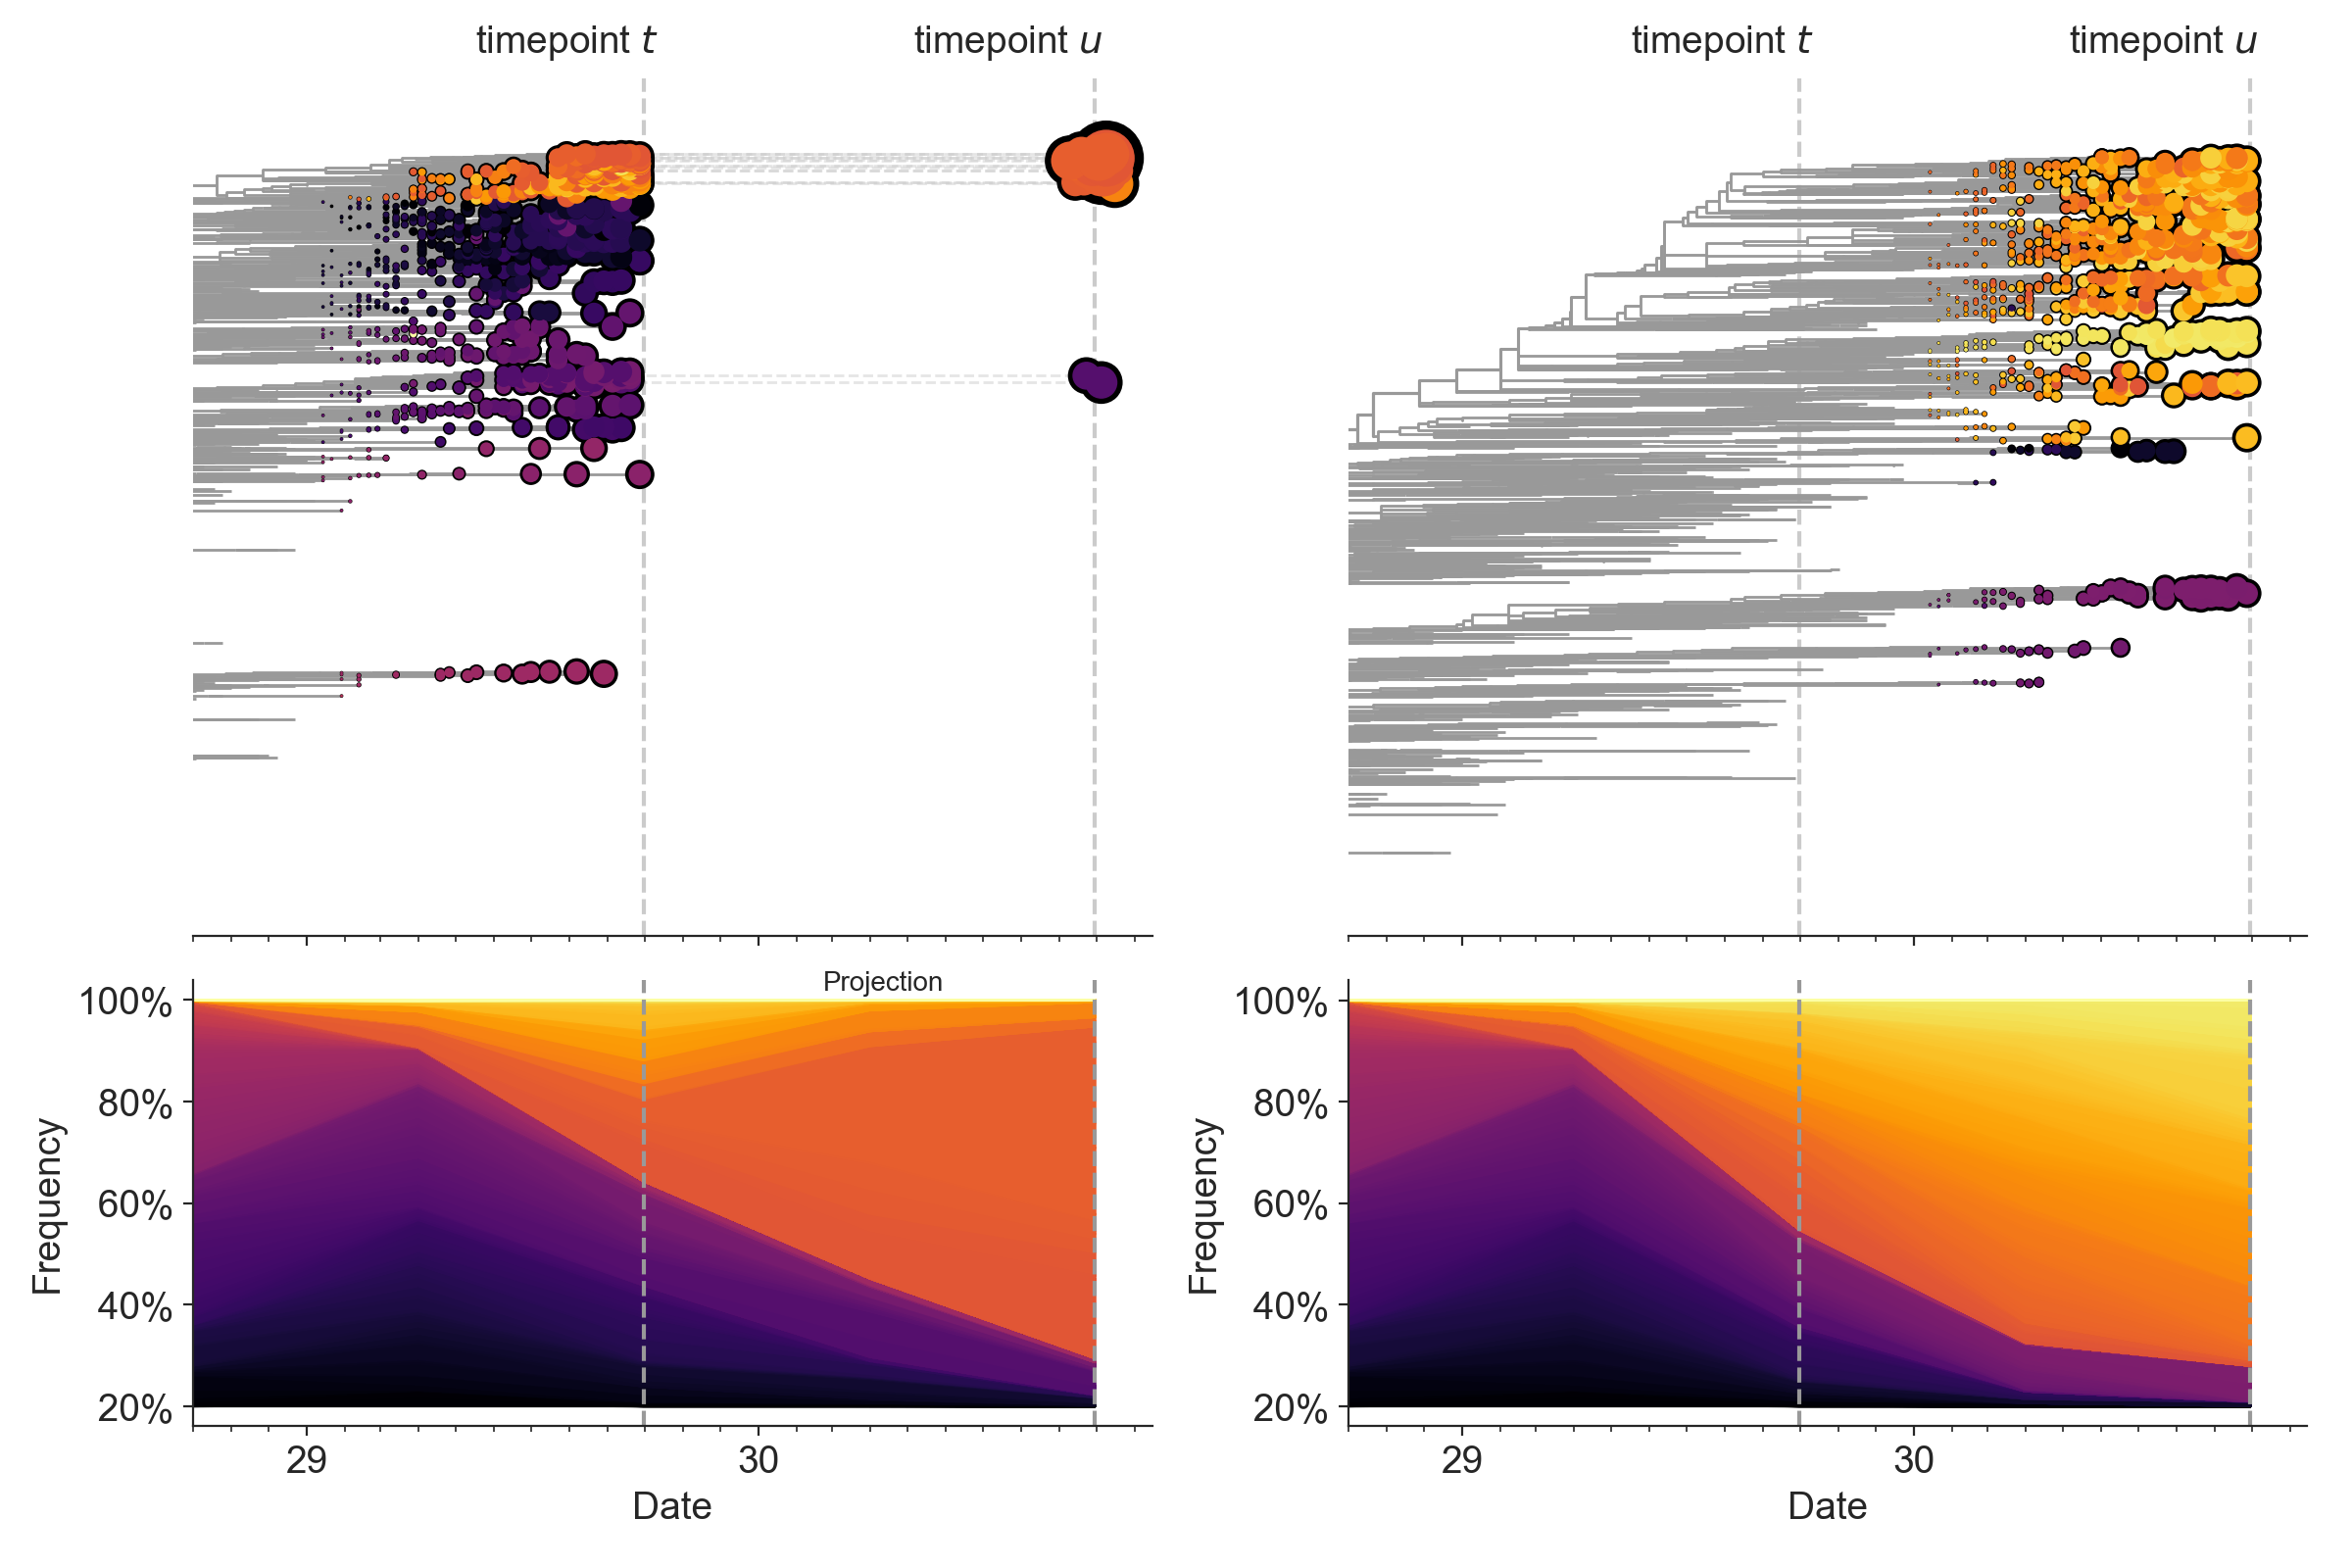
\includegraphics[width=\columnwidth]{figures/distance-based-fitness-model.png}
  \caption{
    Schematic representation of the fitness model for simulated A/H3N2-like populations wherein the fitness of samples at timepoint $t$ determines the estimated frequency of samples with similar sequences one year in the future at timepoint $u$.
    Samples are colored by their amino acid sequence composition such that genetically similar samples have similar colors.
    A) Samples at timepoint $t$ are shown in their phylogenetic context and sized by their frequency at that timepoint.
    The estimated future population at timepoint $u$ is projected to the right with samples scaled in size by their projected frequency based on the true fitness model.
    B) The frequency trajectories of samples at timepoint $t$ to $u$ represent the predicted the growth of the orange samples to the detriment of the purple samples.
    C) Samples at timepoint $u$ are shown in the corresponding phylogeny for that timepoint and scaled by their frequency at that time.
    D) The observed frequency trajectories of samples at timepoint $u$ broadly recapitulate the model's forecasts while also revealing increased diversity of sequences at the future timepoint that the model could not anticipate (e.g., the emergence of the yellow cluster from within the successful orange cluster).
  }
  \label{fig:model}
  \end{center}
\end{figure*}

Here, we present a model of seasonal influenza evolution inspired by the exponential growth model of {\L}uksza and L\"assig \cite{Luksza:2014hj}.
As with this original model, we seek to forecast the frequencies of viral populations one year in advance by applying to each virus sample an exponential growth factor scaled by an estimate of the sample's fitness (Fig.~\ref{fig:model}).
We estimate the frequency of virus samples every six months using a smoothed KDE kernel to represent the frequency of each sample.
We estimate viral fitness with biologically-informed metrics including those originally defined by \cite{Luksza:2014hj} of epitope cross-immunity and non-epitope mutations as well as four more recent metrics including hemagglutination inhibition (HI) cross-immunity \cite{Neher:2016hy}, deep mutational scanning (DMS) mutational effects \cite{Lee2018}, local branching index (LBI) \cite{Neher:2014eu}, and change in clade frequency over time (delta frequency).
We fit models by learning coefficients for each fitness metric either individually or in linear combinations from training data and select the best of these models using time-series cross-validation.
After selecting optimal models from training and validation, we evaluate the true out-of-sample errors of these models on additional data that were held out from the initial model fitting and tuning.
Importantly, our models find fitness coefficients that minimize the normalized average Hamming distance between the observed population one year in the future and the estimated population produced by the exponential growth model (Fig.~\ref{fig:model}).
With this approach, we avoid the intrinsic instability of clade definitions due to variability in phylogenetic reconstruction from year to year.
However, we retain the benefits of fitting models to highly similar samples found within clades and enable future forecasting efforts for pathogens whose sequences are not amenable to standard phylogenetic inference.

\subsection*{Models accurately forecast evolution of A/H3N2-like viruses}

The long-term evolution of influenza A/H3N2 hemagglutinin has been previously described as a balance between positive selection for substitutions that enable escape from adaptive immunity by modifying existing epitopes and purifying selection on domains that are required to maintain the protein's primary functions of binding and membrane fusion \cite{Bush:1999vj,Neher2013,Luksza:2014hj,Koelle:2015dh}.
To test the ability of our models to accurately detect these evolutionary patterns under controlled conditions, we simulated the long-term evolution of A/H3N2-like viruses under positive and purifying selection for 40 years (Methods).
These selective constraints produced phylogenetic structures and accumulation of epitope and non-epitope mutations that were consistent with phylogenies of natural A/H3N2 HA (Supplemental Figure \ref{sup_fig:simulated_h3n2_ha_phylogeny}).
We fit models to these simulated populations using all sequence-only fitness metrics.

We hypothesized that fitness metrics associated with viral success such as epitope cross-immunity, LBI, and delta frequency would be assigned positive coefficients, while metrics associated with fitness penalties, like non-epitope mutations, would receive negative coefficients.
We reasoned that both LBI and delta frequency would individually outperform the mechanistic metrics as both of these growth metrics estimate recent clade success regardless of the mechanistic basis for that success.
Correspondingly, we expected that a composite model of epitope cross-immunity and non-epitope mutations would perform as well as or better than the growth metrics.
In addition to these four estimates of viral fitness, we tested models based on both the true fitness of each sample as measured by the simulator and a naive model under which the exponential growth factor is set to one and populations do not change composition over the one year forecasting period.
The distances estimated under the naive model represent the average distance between the current and future timepoints.

\begin{figure*}[ht]
  \begin{center}
  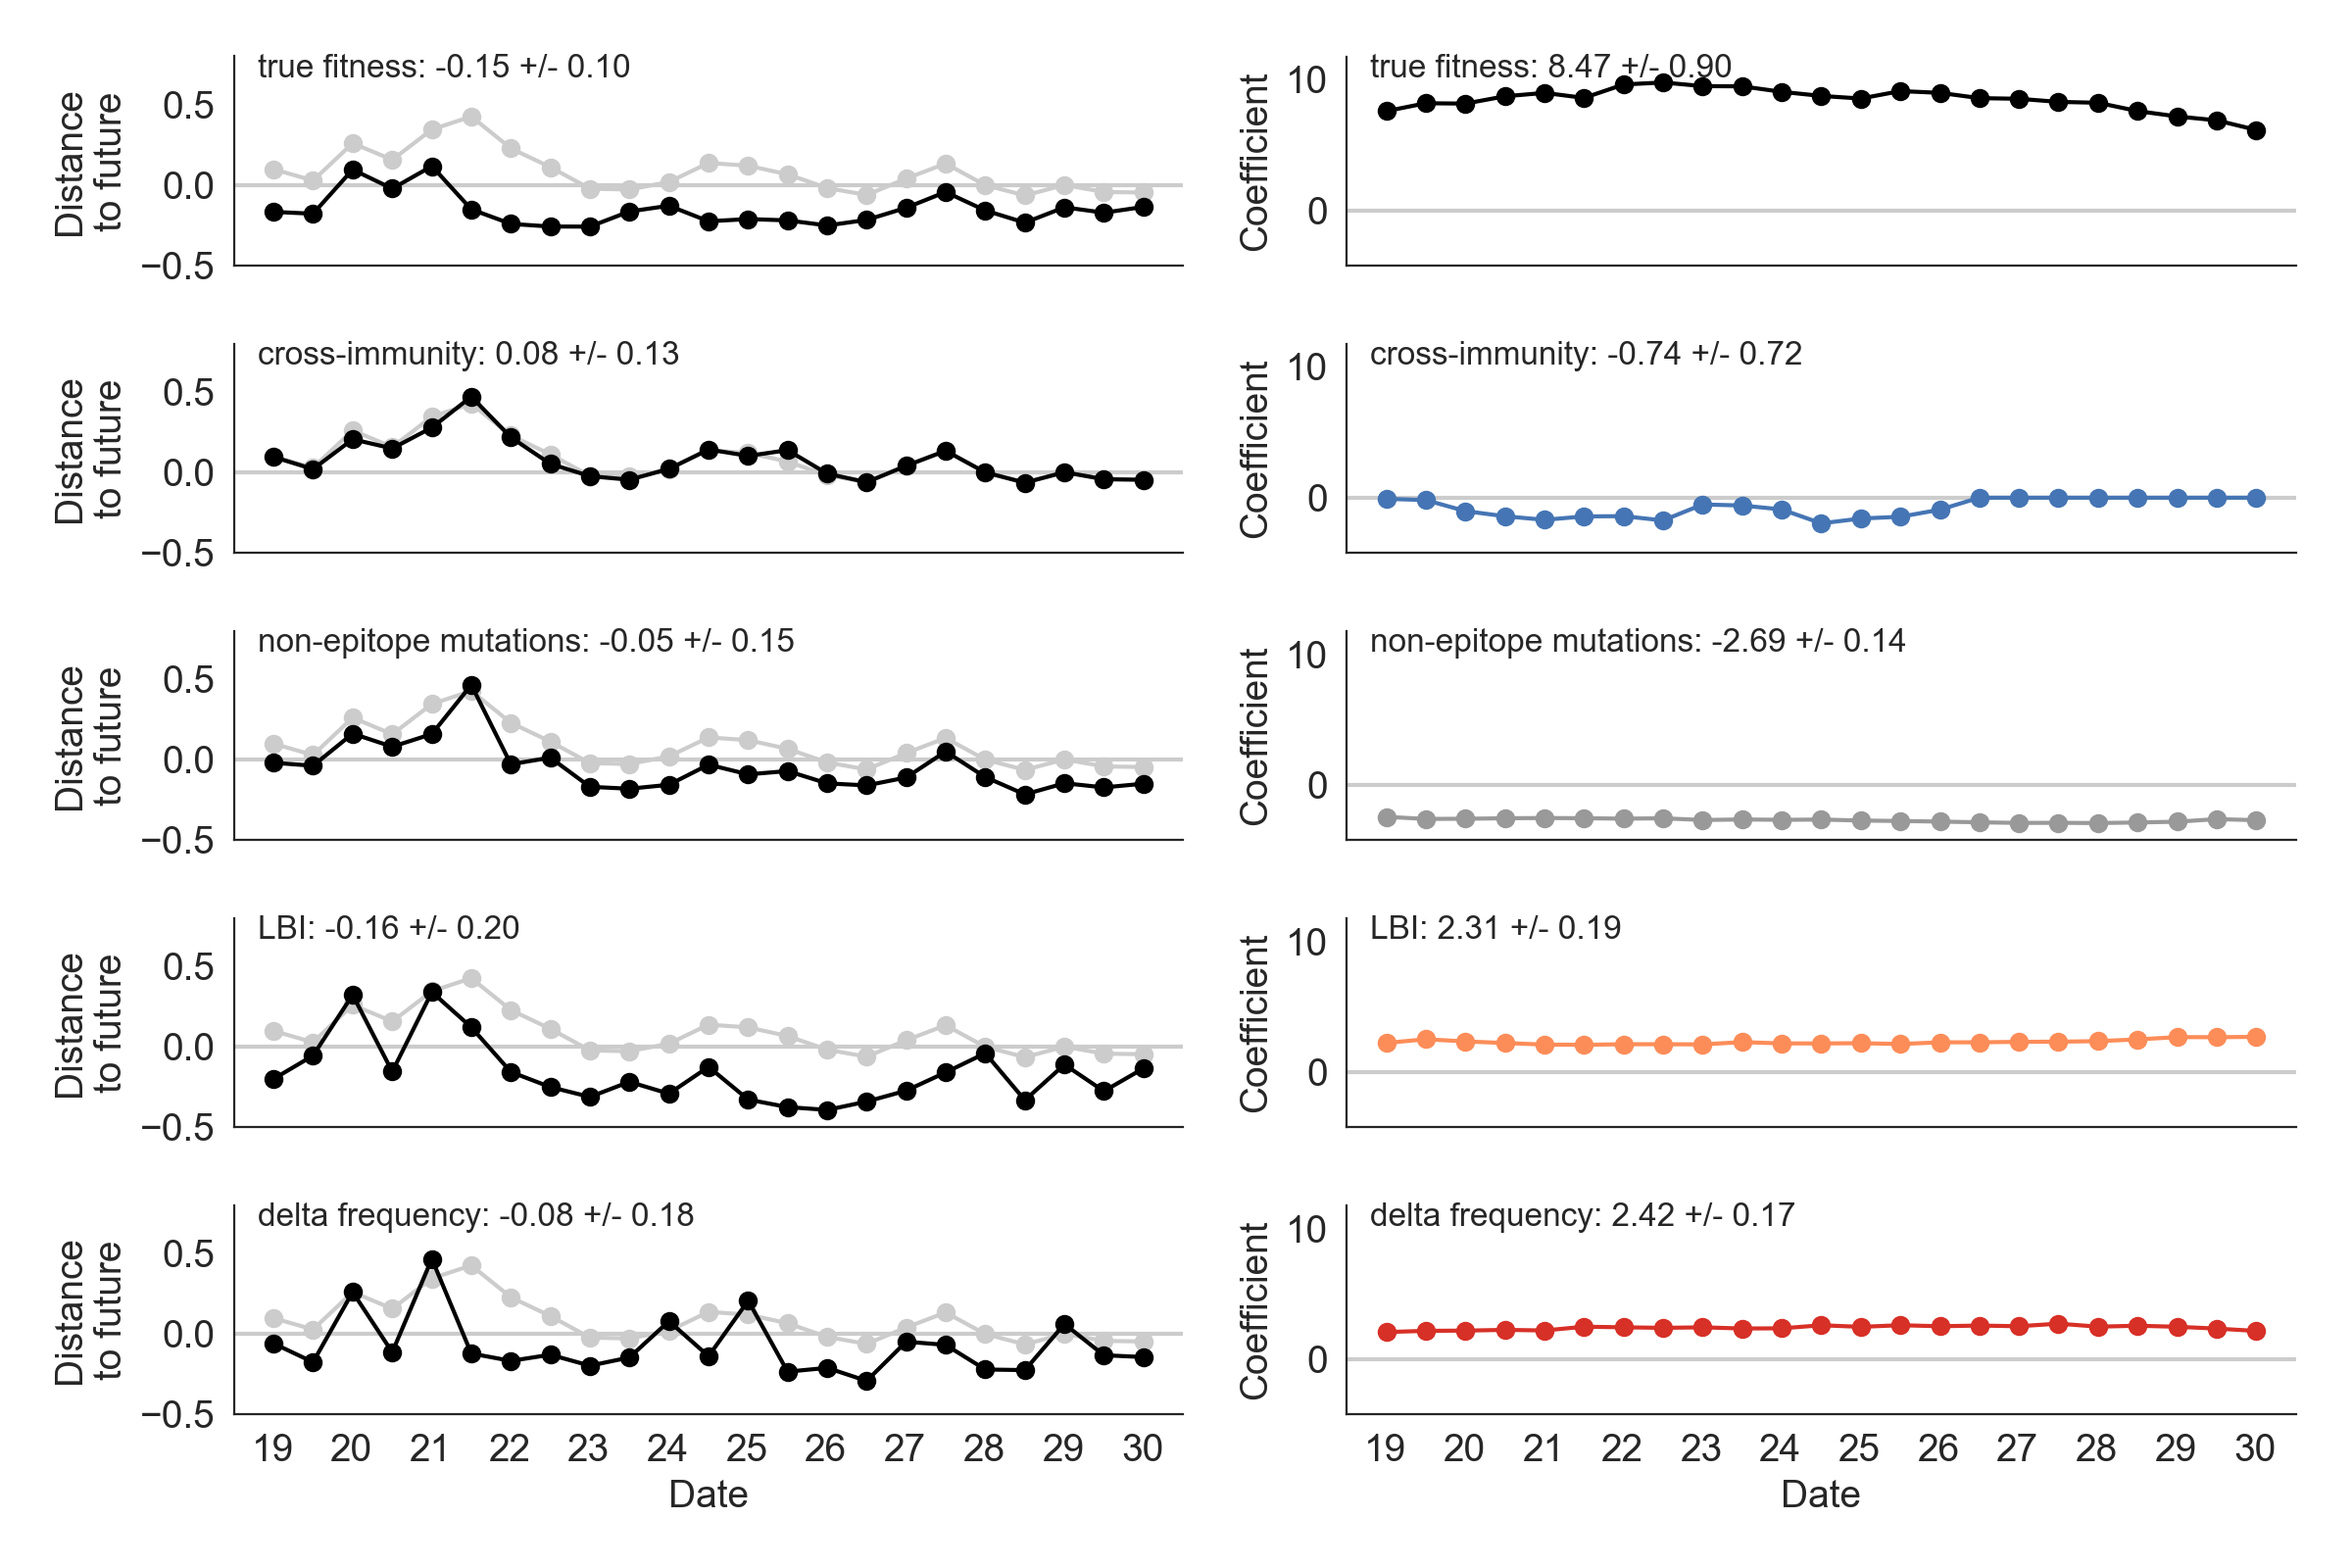
\includegraphics[width=\textwidth]{figures/unadjusted-model-accuracy-and-coefficients-for-simulated-populations.png}
  \caption{
    Model a) coefficients and b) accuracy for simulated populations of A/H3N2-like viruses.
    Coefficients are shown for each individual fitness metric per validation timepoint (N=33) with the mean $\pm$ standard deviation in the top-left corner of each panel.
    Distances to the future in amino acids are shown per validation timepoint for each individual model (black) in the context of the observed distance between timepoints from the naive model (grey).
    Models outperform the naive model when the model's distance to the future is less than the naive model.
    The mean $\pm$ standard deviation of amino acids per timepoint are shown in the top-left of each panel for both the model and the naive model.
  }
  \label{fig:unadjusted_model_accuracy_and_coefficients_for_simulated_populations}
  \end{center}
\end{figure*}

\begin{table*}[ht]
  \begin{center}
    
\begin{tabular*}{1.1\textwidth}{lrllrr}
\toprule
        &                 & \multicolumn{2}{c}{Distance to future (AAs)} & \multicolumn{2}{c}{Model $>$ naive} \\
  Model &    \makecell{Coefficients} & \makecell{Validation} & \makecell{Test} & \makecell{Validation} & \makecell{Test} \\
\midrule

true fitness & 9.37 +/- 0.92 & 6.82 +/- 1.52* & 7.38 +/- 1.89* & 32 (97\%) & 16 (89\%) \\
LBI & 1.31 +/- 0.33 & 7.24 +/- 1.66* & 7.10 +/- 1.19* & 32 (97\%) & 18 (100\%) \\
\hspace{5mm} + mutational load & -1.77 +/- 0.49 & & & & \\
LBI & 2.26 +/- 1.06 & 7.57 +/- 1.85* & 7.51 +/- 1.20* & 29 (88\%) & 17 (94\%) \\
delta frequency & 1.46 +/- 0.44 & 8.13 +/- 1.44* & 8.65 +/- 1.99 & 26 (79\%) & 13 (72\%) \\
epitope ancestor & 0.35 +/- 0.07 & 8.20 +/- 1.39* & 8.17 +/- 1.52* & 29 (88\%) & 17 (94\%) \\
\hspace{5mm} + mutational load & -1.57 +/- 0.13 & & & & \\
mutational load & -1.49 +/- 0.12 & 8.27 +/- 1.35* & 8.20 +/- 1.50* & 29 (88\%) & 17 (94\%) \\
epitope antigenic novelty & 0.03 +/- 0.19 & 8.33 +/- 1.35* & 8.22 +/- 1.51* & 28 (85\%) & 17 (94\%) \\
\hspace{5mm} + mutational load & -1.38 +/- 0.39 & & & & \\
epitope ancestor & 0.14 +/- 0.11 & 8.96 +/- 1.35 & 9.03 +/- 1.68 & 20 (61\%) & 13 (72\%) \\
naive & 0.00 +/- 0.00 & 8.97 +/- 1.35 & 9.07 +/- 1.70 & 0 (0\%) & 0 (0\%) \\
epitope antigenic novelty & -0.03 +/- 0.19 & 9.03 +/- 1.37 & 9.07 +/- 1.69 & 14 (42\%) & 7 (39\%) \\

\bottomrule
\end{tabular*}

    \caption{Simulated population model accuracy relative to the naive model}
    \label{table_simulated_model_selection}
  \end{center}
\end{table*}

The average distance between yearly populations, as measured by the naive model, was 8.97 $\pm$ 1.35 amino acids (Supplemental Fig.~\ref{sup_fig:distance_of_simulated_populations_between_timepoints}).
As expected, the true fitness model outperformed all other models reducing the distance between populations by 2.17 amino acids on average and surpassing the naive model in 32 of 33 (97\%) timepoints (Table~\ref{table_simulated_model_selection} and Fig.~\ref{fig:unadjusted_model_accuracy_and_coefficients_for_simulated_populations}).
With the exception of epitope cross-immunity, all biologically-informed models also outperformed the naive model.
LBI was the best of these models, reducing the distance between populations by 1.41 amino acids on average.
Indeed, both growth-based models received positive coefficients and outperformed the mechanistic models.
The non-epitope mutations metric received a consistently negative coefficient with an average improvement of 0.71 amino acids.
Surprisingly, the composite model of epitope cross-immunity and non-epitope mutations did not perform better than the individual non-epitope mutations model (Supplemental Fig.~\ref{sup_fig:unadjusted_composite_model_accuracy_and_coefficients_for_simulated_populations}).
From these results, we concluded that our method can accurately estimate the evolution of simulated populations, but that the fitness of samples under our simulated conditions was dominated by purifying selection rather than by positive selection at epitope sites.

We hypothesized that a composite model of mutually beneficial metrics could better approximate the true fitness of simulated viruses.
To this end, we fit an additional model including both LBI and non-epitope mutations.
This composite model outperformed all individual metrics, reducing the distance between populations by 1.76 amino acids and outperforming the naive model as often as the true fitness metric (Fig.~\ref{fig:unadjusted_model_accuracy_and_coefficients_for_simulated_populations}).
Interestingly, we found that the coefficients for LBI and non-epitope mutations remained relatively stable across all validation timepoints.
These results support our hypothesis that multiple complementary metrics can produce more accurate models.

Finally, we sought to validate and test the best performing model by two metrics relevant for practical influenza forecasting and vaccine design efforts.
First, we measured the ability of the true fitness model to accurately estimate clade dynamics by correlating estimated and observed clade growth rates.
Under these simulated conditions, our model satisfactorily recapitulated clade dynamics with a growth rate correlation of $R = 0.71 (p < 0.001)$ and overall accuracies for clade growth and decline predictions of 66\% and 61\%, respectively (Supplemental Fig.~\ref{sup_fig:validation_of_best_model_for_simulated_populations}A).
Next, we tested how often the estimated closest strain to the future population at any given timepoint ranked among the observed top closest strains to the future.
The estimated best strain was in the top 4th percentile of observed closest strains for half of the validation timepoints and in the top 20th percentile for 82\% of timepoints (Supplemental Fig.~\ref{sup_fig:validation_of_best_model_for_simulated_populations}B).
These results confirm that our approach of minimizing the distance between yearly populations can simulataneously capture clade-level dynamics of these populations and identify optimal individual strains as vaccine candidates.

\subsection*{Model coefficients and performance reflect historical patterns of A/H3N2 evolution}

Next, we trained and validated models for individual fitness predictors using 23 years of natural A/H3N2 populations spanning from October 1992 to October 2015.
We held out samples collected between October 2015 and April 2019 for model testing.
In addition to the sequence-only models we tested on simulated populations, we also fit models for our new fitness metrics based on experimental phenotypes including HI cross-immunity and DMS mutational effects.
We hypothesized that both HI and DMS metrics would be assigned positive coefficients, as they estimate increased antigenic drift and beneficial mutations, respectively.
As antigenic drift is generally considered to be the primary evolutionary pressure on natural A/H3N2 populations \cite{Smith:2004jc,Bedford:2014bf,Luksza:2014hj}, we expected that epitope and HI cross-immunity would be individually more predictive than non-epitope mutations or DMS mutational effects.
Previous research \cite{Neher:2016hy} and our simulation results also led us to expect that LBI and delta frequency would outperform other individual mechanistic metrics.

\begin{figure*}[ht]
  \begin{center}
  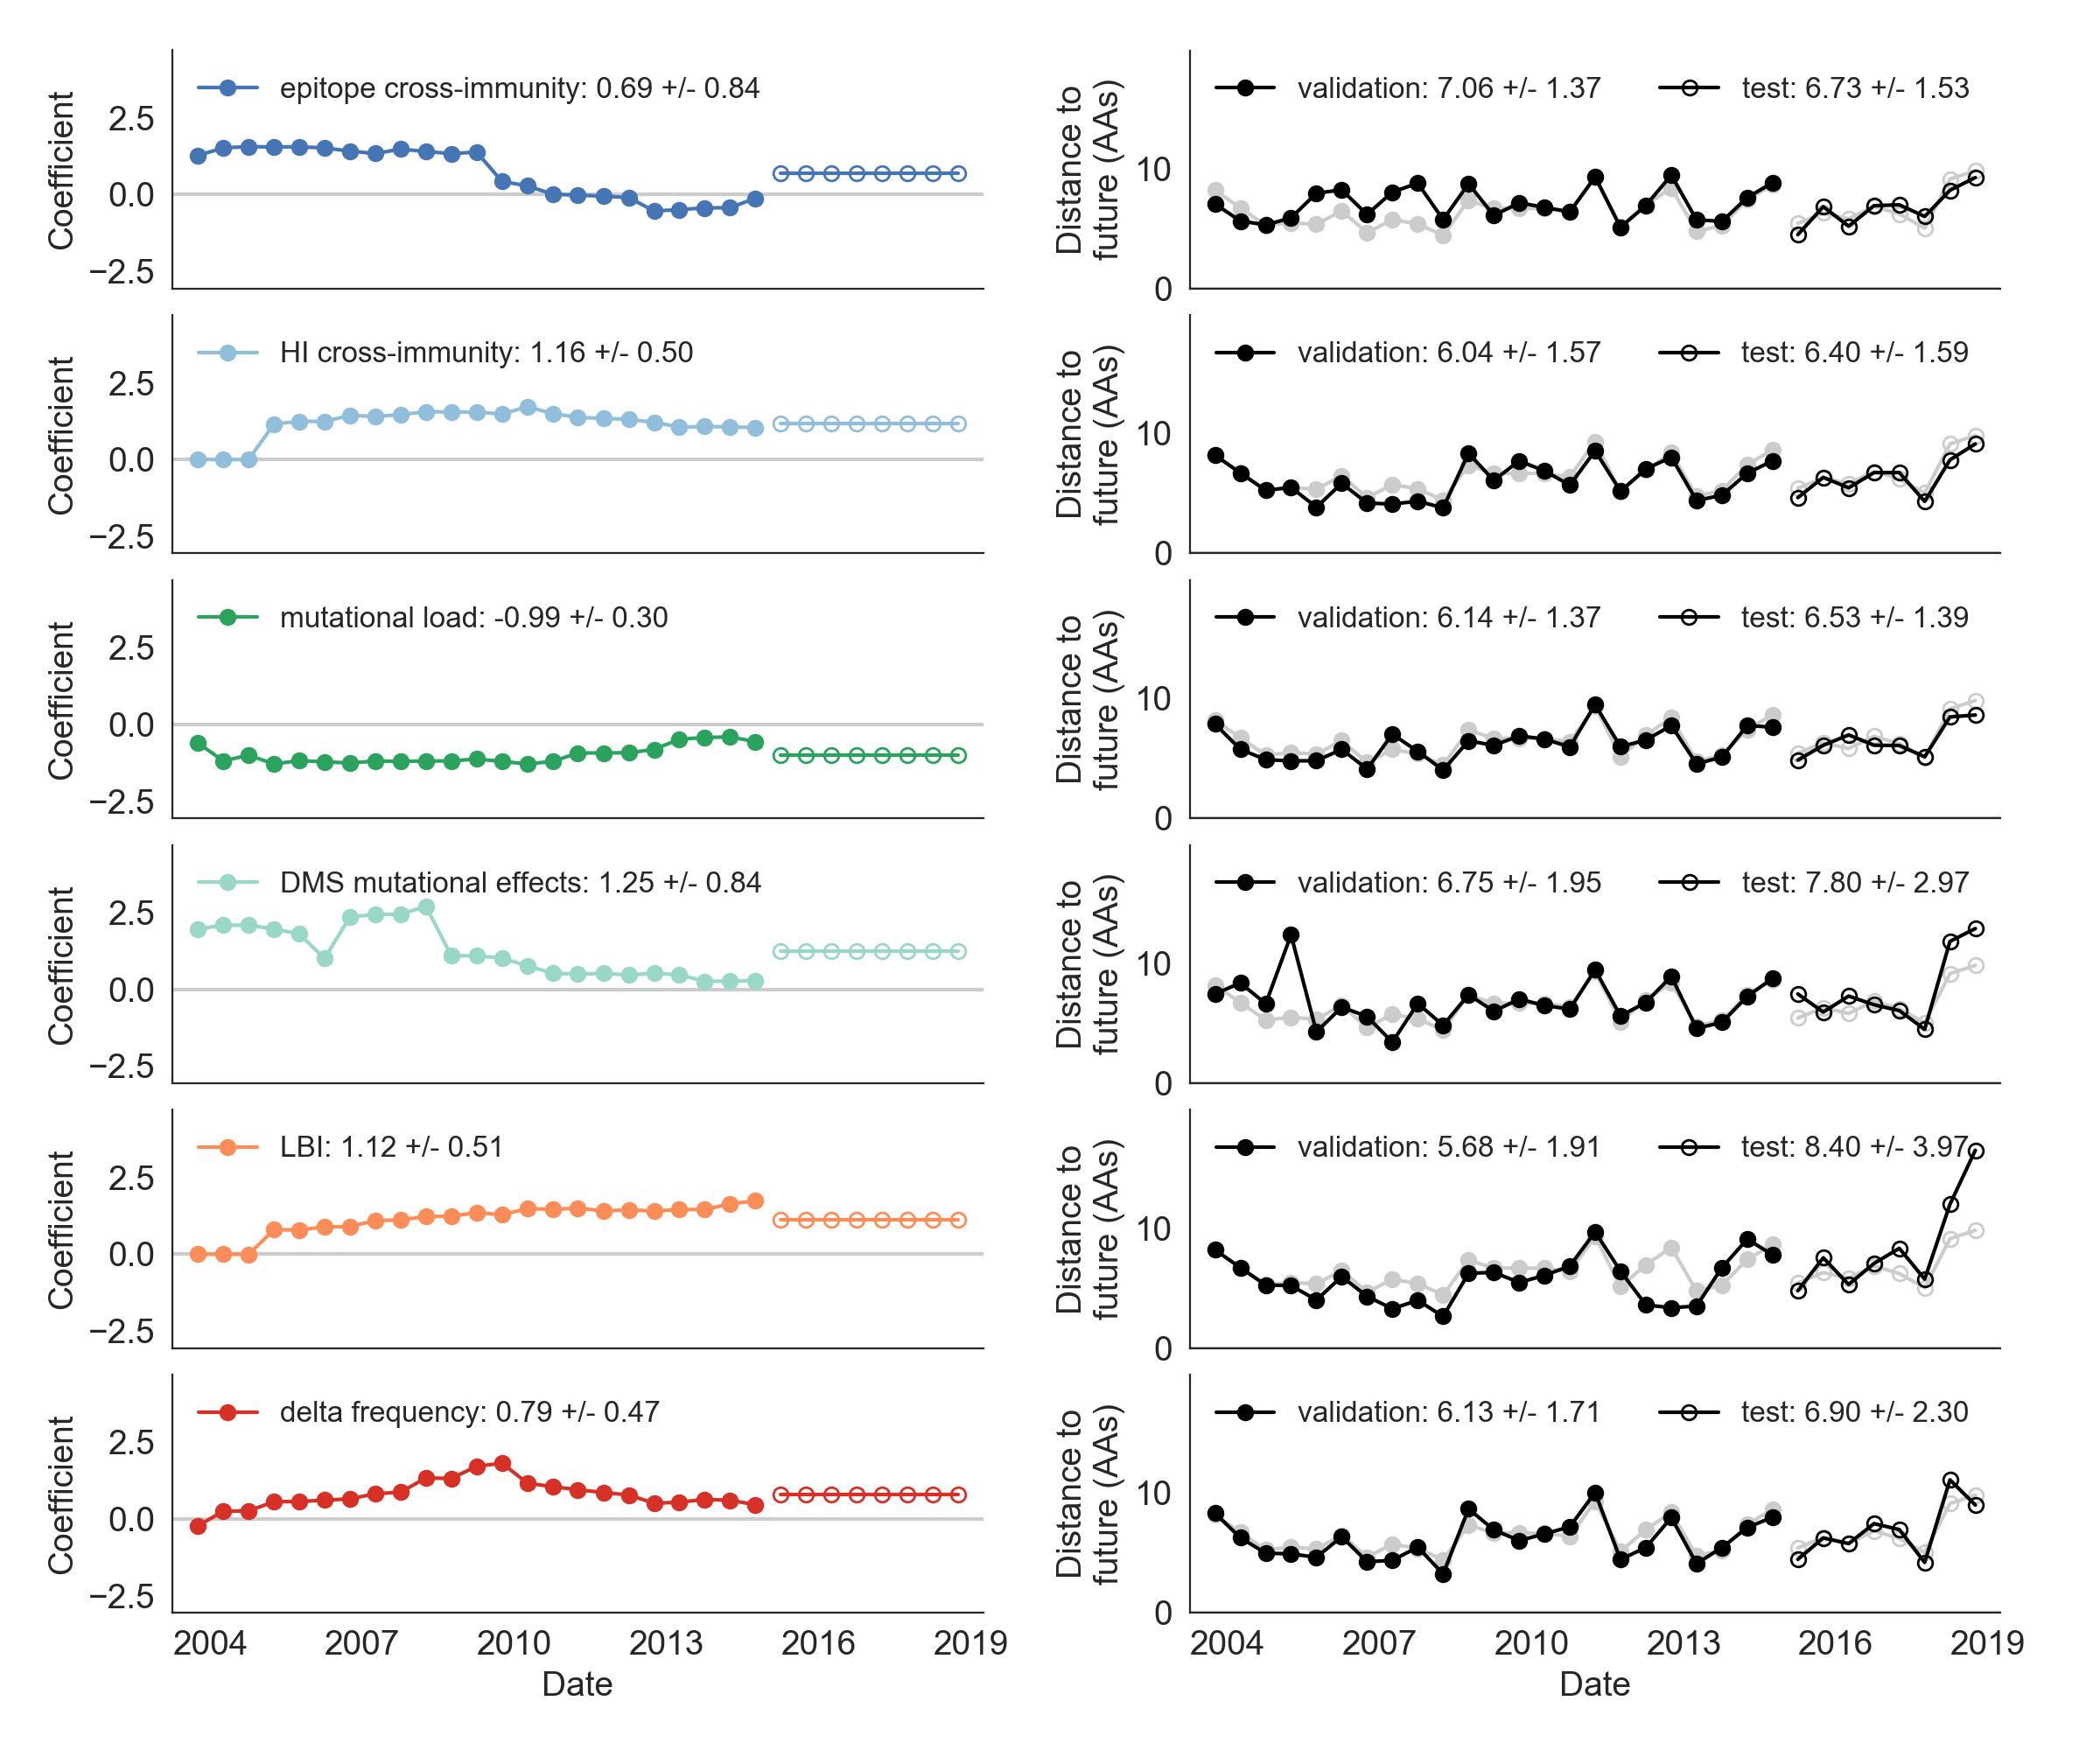
\includegraphics[width=\textwidth]{figures/unadjusted-model-accuracy-and-coefficients-for-natural-populations.png}
  \caption{
    Model a) coefficients and b) accuracy for natural populations of A/H3N2 viruses.
    As in Fig.~\ref{fig:unadjusted_model_accuracy_and_coefficients_for_simulated_populations}, coefficients are shown for each individual fitness metric per validation timepoint (N=19) with the mean $\pm$ standard deviation in the top-left corner of each panel.
    Distances to the future in amino acids are shown per validation timepoint for each individual model (black) in the context of the observed distance between timepoints from the naive model (grey).
    Models outperform the naive model when the model's distance to the future is less than the naive model.
    The mean $\pm$ standard deviation of amino acids per timepoint are shown in the top-left of each panel for both the model and the naive model.
  }
  \label{fig:unadjusted_model_accuracy_and_coefficients_for_natural_populations}
  \end{center}
\end{figure*}

\begin{table*}[ht]
  \begin{center}
    
\begin{tabular*}{1.05\textwidth}{lrrrrr}
\toprule
        &                 & \multicolumn{2}{c}{Distance to future (AAs)} & \multicolumn{2}{c}{Model $>$ naive} \\
  Model &    \makecell{Coefficients} & \makecell{Validation} & \makecell{Test} & \makecell{Validation} & \makecell{Test} \\
\midrule

mutational load & -0.68 +/- 0.34 & 5.44 +/- 1.80 & 7.70 +/- 3.53 & 18 (78\%) & 4 (50\%) \\
\hspace{5mm} + LBI & 1.03 +/- 0.40 & & & & \\
LBI & 1.12 +/- 0.51 & 5.68 +/- 1.91 & 8.40 +/- 3.97 & 17 (74\%) & 2 (25\%) \\
HI cross-immunity & 1.39 +/- 0.19 & 5.77 +/- 1.53 & 6.16 +/- 1.43 & 18 (78\%) & 6 (75\%) \\
\hspace{5mm} + mutational load & -1.02 +/- 0.45 & & & & \\
HI cross-immunity & 1.28 +/- 0.47 & 5.88 +/- 1.63 & 6.12 +/- 1.42 & 19 (83\%) & 6 (75\%) \\
\hspace{5mm} + mutational load & -1.03 +/- 0.53 & & & & \\
\hspace{5mm} + LBI & 0.05 +/- 0.50 & & & & \\
HI cross-immunity & 1.16 +/- 0.50 & 6.04 +/- 1.57 & 6.40 +/- 1.59 & 17 (74\%) & 6 (75\%) \\
delta frequency & 0.79 +/- 0.47 & 6.13 +/- 1.71 & 6.90 +/- 2.30 & 16 (70\%) & 5 (62\%) \\
mutational load & -0.99 +/- 0.30 & 6.14 +/- 1.37 & 6.53 +/- 1.39 & 17 (74\%) & 6 (75\%) \\
naive & 0.00 +/- 0.00 & 6.40 +/- 1.36 & 6.82 +/- 1.74 & 0 (0\%) & 0 (0\%) \\
DMS mutational effects & 1.25 +/- 0.84 & 6.75 +/- 1.95 & 7.80 +/- 2.97 & 11 (48\%) & 4 (50\%) \\
epitope cross-immunity & 0.69 +/- 0.84 & 7.06 +/- 1.37 & 6.73 +/- 1.53 & 6 (26\%) & 4 (50\%) \\

\bottomrule
\end{tabular*}

    \caption{Natural population model accuracy relative to the naive model}
    \label{table_natural_model_selection}
  \end{center}
\end{table*}

The average distance per year between natural populations was 6.50 $\pm$ 1.42 amino acids or 72\% of the distance between yearly simulated populations (Supplemental Fig.~\ref{sup_fig:distance_of_natural_populations_between_timepoints}).
Biologically-informed metrics generally performed better than the naive model for natural populations with the exceptions of the epitope cross-immunity and DMS mutational effects (Fig.~\ref{fig:unadjusted_model_accuracy_and_coefficients_for_natural_populations}).
Surprisingly, the best antigenic fitness metric of HI cross-immunity performed only slightly better the best functional constraint metric of non-epitope mutations.
Indeed, epitope cross-immunity only outperformed the naive model at one of 19 timepoints (5\%), while HI cross-immunity outperformed the naive model at 15 (79\%) timepoints (Table~\ref{table_natural_model_selection}).
Epitope cross-immunity was also the only metric whose coefficient started at a positive value and transitioned to a negative value through the validation period.
This change in coefficient suggests that positive selection may have weakened at these epitope sites over time.
In contrast, HI cross-immunity maintained a positive coefficient across most timepoints.
The HI cross-immunity may benefit from being able to constantly update its antigenic model at each timepoint with recent experimental phenotypes, while the epitope cross-immunity metric is forced to give a constant weight to the same 49 sites throughout time.

Non-epitope mutations also outperformed the DMS mutational effects, reducing the distance to the future by 0.40 amino acids on average compared to 0.19 amino acids, respectively.
In contrast to the original {\L}uksza and L\"assig \cite{Luksza:2014hj} model, where the coefficient of the non-epitope mutations metric was fixed at -0.5, our model learned a consistently stronger coefficient of -1.45 $\pm$ 0.24.
Notably, DMS mutational effects only performed noticeably better than the naive model at the timepoint immediately preceding when the background strain of the DMS experiments, A/Perth/16/2009, was sampled.
This result is consistent with the DMS model overfitting to the evolutionary history of the background strain used to perform the DMS experiments.
Alternate implementations of less background-dependent DMS metrics never performed better than the non-epitope mutations metric (Supplemental Fig.~\ref{sup_fig:unadjusted_DMS_model_accuracy_and_coefficients_for_natural_populations}).
Thus, we find that a simple model where any mutation at non-epitope sites is deleterious is more predictive of global viral success than a more comprehensive model based on measured mutational effects.

LBI was the best individual fitness metric by average distance to the future (Fig.~\ref{fig:unadjusted_model_accuracy_and_coefficients_for_natural_populations}).
However, LBI only outperformed the naive model 63\% of the time (Table~\ref{table_natural_model_selection}).
These results suggest that when LBI forecasts correctly, it does so better than other metrics, but that it is prone to overfitting.
Delta frequency did not surpass LBI in average estimated distance to the future and performed worse than both the HI cross-immunity and non-epitope mutation models.
While delta frequency should, in principle, measure the same aspect of viral fitness as LBI, these results clearly show that the current implementations of these metrics represent qualitatively different fitness components.

\subsection*{Composite models outperform models with individual fitness metrics}

To test whether composite models could outperform individual fitness metrics for natural populations, we fit models based on combinations of best individual metrics representing antigenic drift, functional constraint, and clade growth.
Specifically, we fit models based on HI cross-immunity and non-epitope mutations, LBI and non-epitope mutations, and all three of these metrics together.
We anticipated that if these metrics all represented distinct, mutually beneficial components of viral fitness, these composite models should perform better than individual models with consistent coefficients for each metric.

\begin{figure*}[ht]
  \begin{center}
  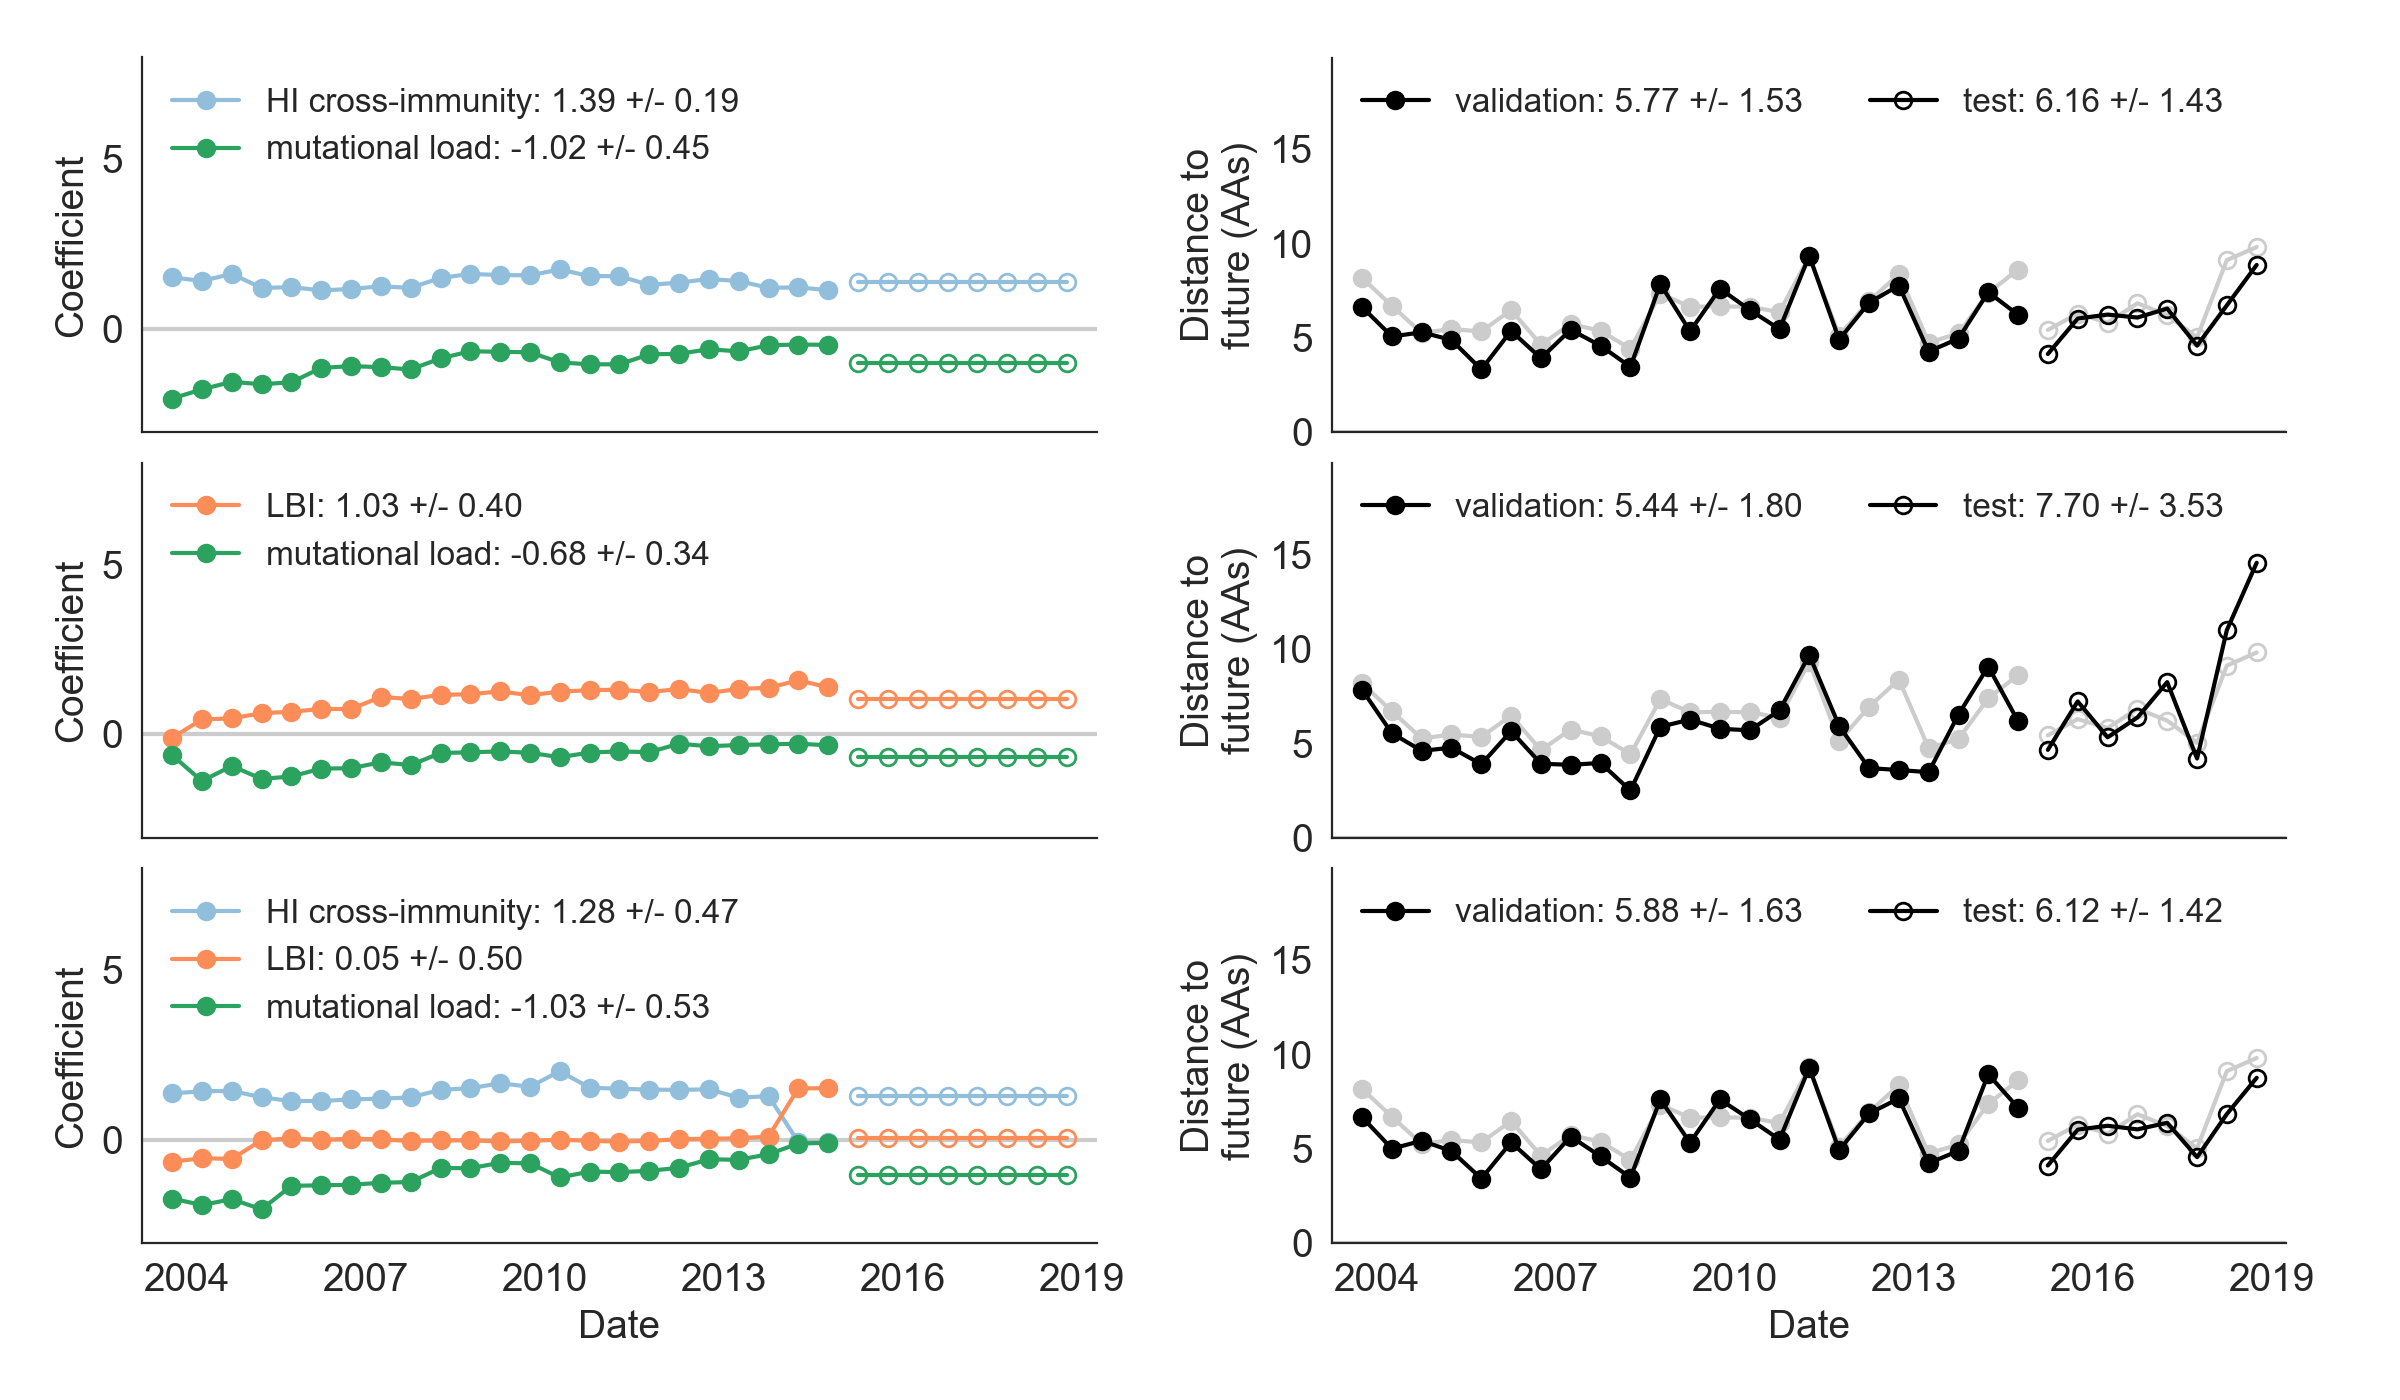
\includegraphics[width=\textwidth]{figures/best-composite-unadjusted-model-accuracy-and-coefficients-for-natural-populations.png}
  \caption{
    Composite model a) accuracy and b) coefficients for natural populations of A/H3N2 viruses.
    As in Fig.~\ref{fig:unadjusted_model_accuracy_and_coefficients_for_natural_populations}, coefficients are shown per timepoint for each individual fitness metric by the corresponding color of the metric.
  }
  \label{fig:unadjusted_composite_model_accuracy_and_coefficients_for_natural_populations}
  \end{center}
\end{figure*}

As expected, all of these composite models performed better than any of their corresponding individual models (Table~\ref{table_natural_model_selection} and Fig.~\ref{fig:unadjusted_composite_model_accuracy_and_coefficients_for_natural_populations}).
The model with all three metrics performed the best, reducing the distance to the future by 1.21 amino acids on average.
This 19\% reduction of distance to the future relative to the naive model was nearly equal to the 20\% relative reduction of the best composite model for simulated populations.
However, the composite of LBI and non-epitope mutations performed nearly as well with an average reduced distance of 1.14.
Both of these models were more accurate than the naive model for 79\% of validation timepoints.
Although the composite of HI cross-immunity and non-epitope mutations outperformed the naive model more often than LBI, this composite model did not reduce the estimated distance to the future better on average than the individual LBI metric.
Indeed, we observed that the contribution of HI cross-immunity to the best composite model declined after October 2010 when that metric's coefficient converged to zero (Fig.~\ref{fig:unadjusted_composite_model_accuracy_and_coefficients_for_natural_populations}).
These results reinforce the historical importance of HI assays in measuring viral fitness, while also indicating that these assays are no longer as predictive as sequence-only metrics.

\subsection*{Models enable selection of vaccine candidate strains}

As with the simulated populations, we validated the performance of the best model for natural populations using estimated and observed clade growth rates and the ranking of estimated best strains compared to the observed closest strains to future populations.
We find that the composite model of LBI and non-epitope mutations capture clade decline with 94\% accuracy and modestly reflects observed clade growth with 66\% accuracy (Fig.~\ref{fig:validation_of_best_model_for_natural_populations}A).


\begin{figure*}[ht]
  \begin{center}
  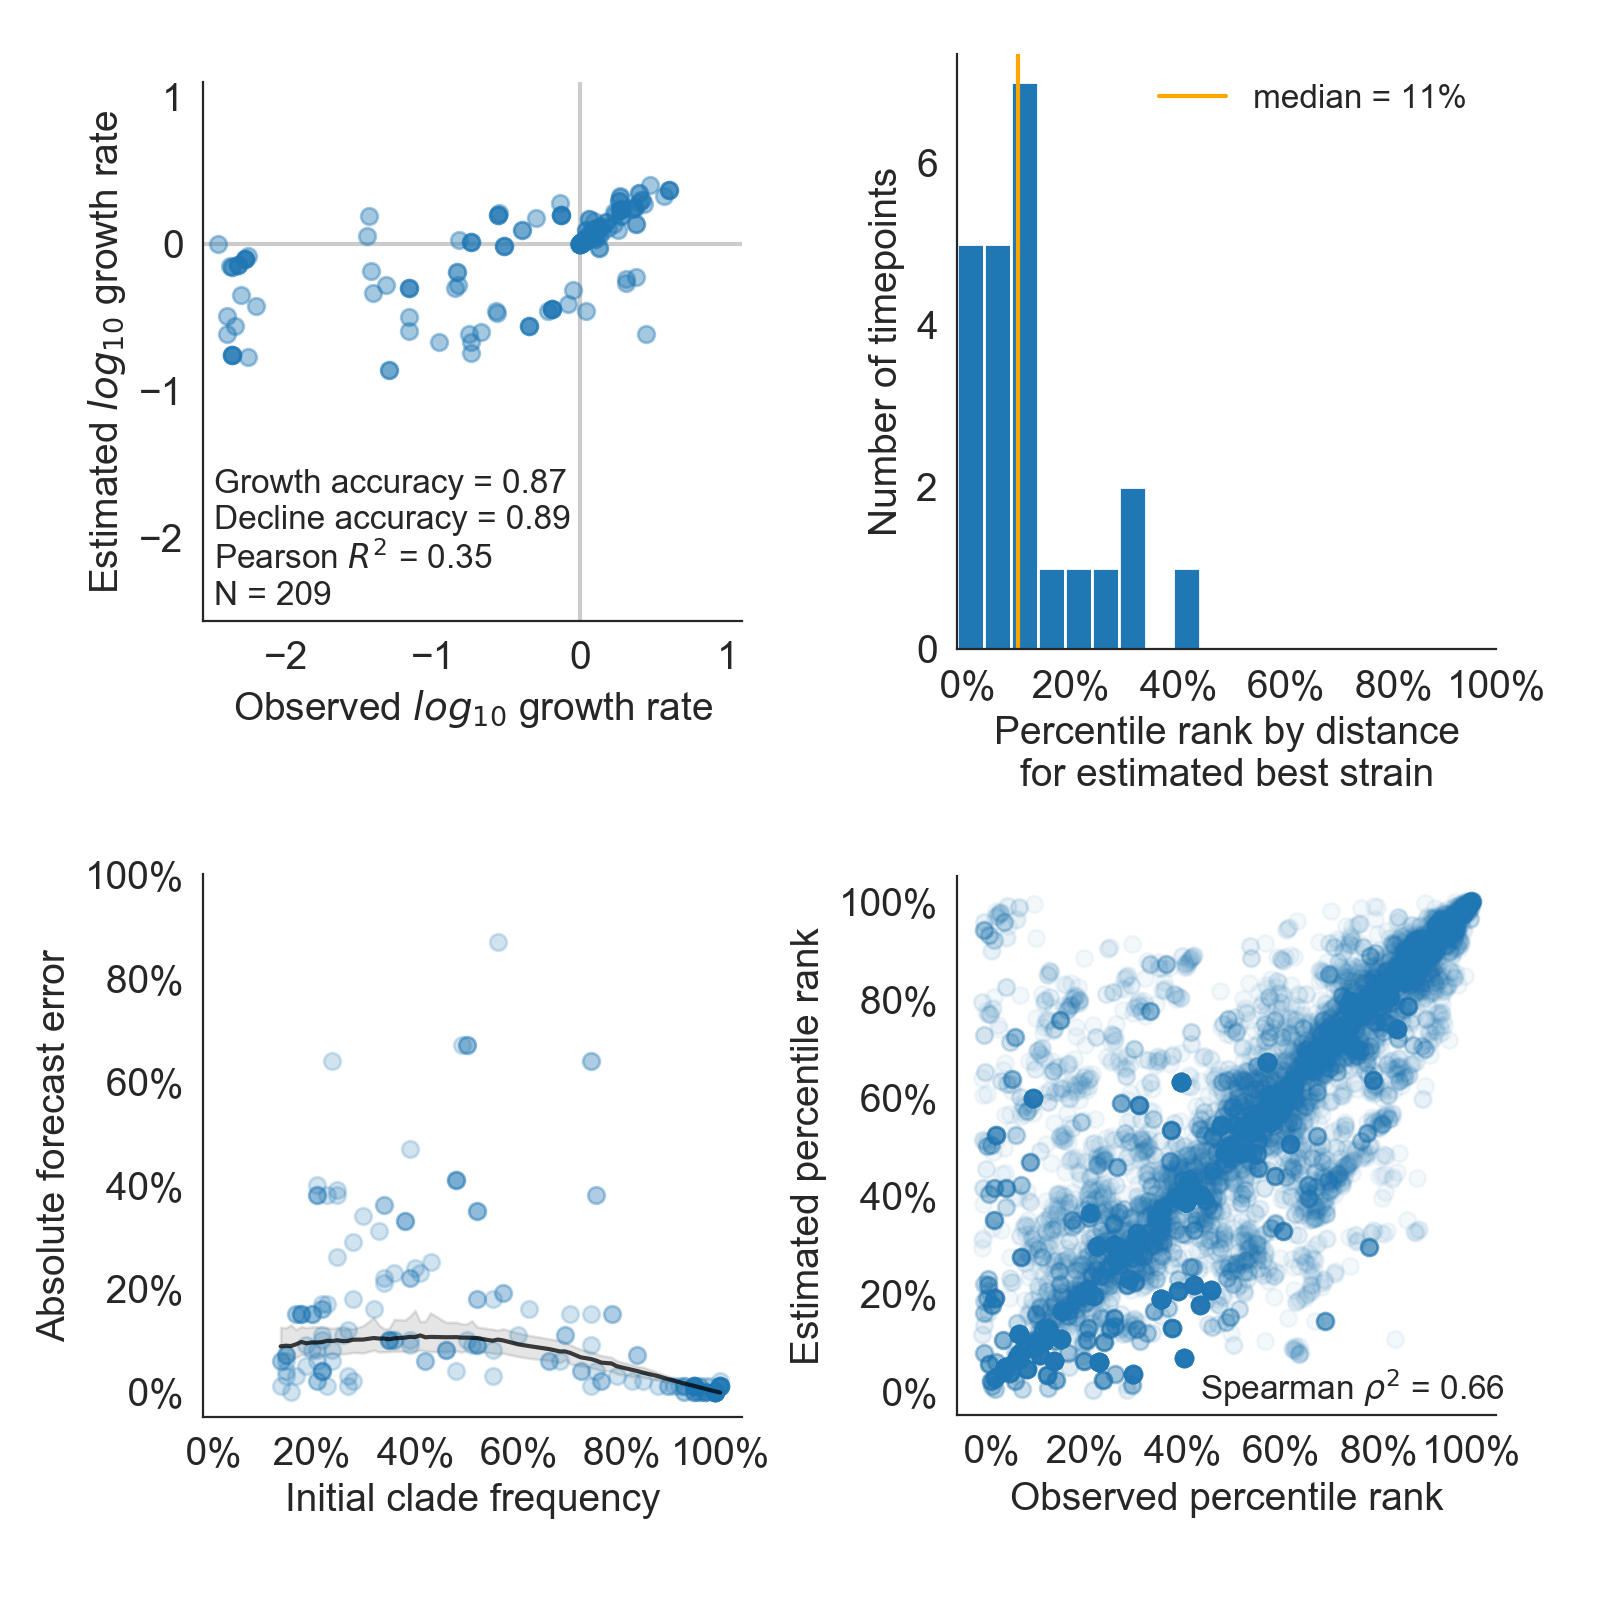
\includegraphics[width=\textwidth]{figures/validation-of-best-model-for-natural-populations.png}
  \caption{
  Validation of best model for natural populations of A/H3N2 viruses, the composite model of LBI and non-epitope mutations.
  A) The correlation of estimated and observed clade growth rates shows the model's ability to capture clade-level dynamics without explicitly optimizing for clade frequency targets.
  B) The rank of the estimated best strain based on its distance to the future in the best model shows how often the model makes a good choice when forced to select a single representative strain for the future population.
  }
  \label{fig:validation_of_best_model_for_natural_populations}
  \end{center}
\end{figure*}

\subsection*{Forecasts predict the rise of A1b/131K and A1b/135K sub-clades in September 2020}

See Fig.~\ref{fig:nextstrain_forecasts}.

\begin{figure*}[ht]
  \begin{center}
  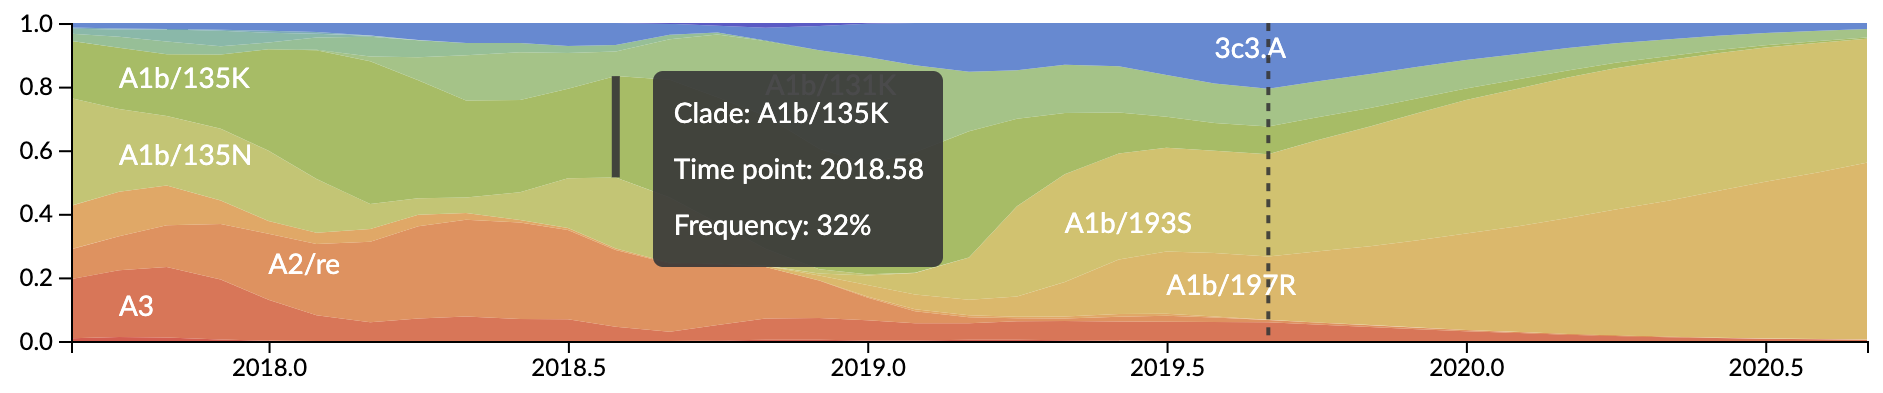
\includegraphics[width=\textwidth]{figures/nextstrain-forecasts-for-september-2020.png}
  \caption{
    Snapshot of live forecasts on nextstrain.org from our best model for September 2020.
    The observed frequency trajectories for currently circulating clades are shown up to September 2019.
    Our model favors the A1b/131K subclade, A1b/197R, to grow over the next year and estimates that the A1b/135K subclade, A1b/137F, will remain stable.
  }
  \label{fig:nextstrain_forecasts}
  \end{center}
\end{figure*}

\section*{Discussion}

\begin{itemize}
\item{Our model accurate forecasts evolution of simulated and natural populations by estimating the sequence composition of future populations and without relying on clade-based model targets}
\item{The combination of sequence-only metrics outperforms all experimentally-informed metrics}
\item{Deleterious mutations contribute more to seasonal influenza evolution than has been as widely appreciated}
\item{Epitope mutations are an inadequate predictor of viral success compared to other antigenic or phylogenetic metrics}
\item{Further efforts to understand the declining efficacy of HI assays and to replace these with FRA or antigenic escape assays could improve models in the future}
\item{Our model live forecasts in nextstrain.org will aid in year-round surveillance of influenza evolutionary patterns and allow us to continuously evaluate model performance relative to recent observations}
\item{Our model is the first of its kind to be released as an open source framework that can be inspected and extended by others}
\item{Immediate next steps to improve influenza models under this framework include the integration of geographic information and antigenic escape assay data}
\item{Our distance-based model targets and easy definition of fitness metrics through tidy data frames paves the way for future forecasting efforts with pathogens that cannot be analyzed by standard phylogenetic methods (e.g., highly recombinant viruses and organisms with larger genomes like bacteria and fungi)}
\end{itemize}

\section*{Methods}

\subsection*{Simulation of influenza A/H3N2-like populations}

We simulated the long-term evolution of A/H3N2-like viruses with SANTA-SIM \cite{Jariani2019} for 50 years where 200 generations was equivalent to 1 year.
We discarded the first 10 years as a burn-in period, selected the next 30 years for model fitting and validation, and held out the last 10 years as out-of-sample data for model testing.
Each simulated population was seeded with the full length HA from A/Beijing/32/1992 (NCBI accession: U26830.1) such that all simulated sequences contained signal peptide, HA1, and HA2 domains.
We defined purifying selection across all three domains, allowing the preferred amino acid at each site to change at a fixed rate over time.
We additionally defined exposure-dependent selection for 49 putative epitope sites in HA1 \cite{Luksza:2014hj} to impose an effect of cross-immunity that would allow mutations at those sites to increase viral fitness despite underlying purifying selection.
We modified the SANTA-SIM source code to enable the inclusion of true fitness values for each sample in the FASTA header of the sampled sequences from each generation.
This modified implementation is available at \url{https://github.com/huddlej/santa-sim/tree/emit-fitness}.
For our full analysis of model performance, we sampled 90 viruses per month to match the sampling density of natural populations.
For tuning of hyperparameters, we sampled 10 viruses per month to enable rapid exploration of hyperparameter space.

\subsection*{Hyperparameter tuning with simulated populations}

To avoid overfitting our models to the relatively limited data from natural populations, we used simulated A/H3N2-like populations to tune hyperparameters including the KDE bandwidth for frequency estimates and the L1 penalty for model coefficients.
We simulated populations, as described above, and fit models for each parameter value using the true fitness of samples from the simulator.

We identified the optimal KDE bandwidth for frequencies as the value that minimized the difference between the mean distances to the future from the true fitness model and the naive model.
We set the L1 lambda penalty to zero, to reduce variables in the analysis and avoid interactions between the coefficients and the KDE bandwidths.
Higher bandwidths completely wash out dynamics of populations by making all samples appear to exist for long time periods.
This flattening of frequency trajectories means that as bandwidths increase, the naive model gets more accurate and less informative.
Given this behavior, we found the bandwidth that produced the minimum difference between distances to the future for the true fitness and naive models instead of the bandwidth that produced the minimum mean model distance.
Based on this analysis, we identified an optimal bandwidth of $\frac{2}{12}$ or the equivalent of 2-months for floating point dates.
Next, we identified an L1 penalty of 0.1 for model coefficients that minimized the mean distance to the future for the true fitness model.

\subsection*{Strain selection for natural populations}

For model training and validation, we selected 13,568 HA sequences $\geq$900 nucleotides that were sampled between October 1, 1992 and October 1, 2015.
To account for known variation in sequence availability by region, we subsampled the selected sequences to a representative set of 90 viruses per month with even sampling across 10 global regions including Africa, Europe, North America, China, South Asia, Japan and Korea, Oceania, South America, Southeast Asia, and West Asia.
We excluded all egg-passaged samples and all samples with ambiguous year, month, and day annotations.
We prioritized samples with more available HI titer measurements.
For model testing, we selected an additional XX HA sequences that were sampled between October 1, 2015 and April 1, 2019.
We used these test sequences to evaluate the out-of-sample error of fixed model parameters learned during training and validation.

\subsection*{Phylogenetic interference}

For each timepoint in model training, validation, and testing, we selected the subsampled HA sequences with collection dates up to that timepoint.
We aligned sequences with the augur align command \cite{Hadfield2018} and MAFFT v7.407 \cite{Katoh2002}.
We inferred initial phylogenies for HA sequences at each timepoint with IQ-TREE v1.6.10 \cite{Nguyen2014}.
To reconstruct time-resolved phylogenies, we applied TreeTime v0.5.6 \cite{Sagulenko2018} with the augur refine command.

\subsection*{Frequency estimation}

To account for uncertainty in collection date and sampling error, we applied a kernel density estimation (KDE) approach to calculate global sample frequencies.
Specifically, we constructed a Gaussian kernel for each sample with the mean at the reported collection date and a variance (or KDE bandwidth) of two months.
The bandwidth was identified by cross-validation, as described above.
This bandwidth also roughly corresponds to the median lag time between sample collection and submission to the GISAID database.
We estimated the frequency of each sample at each timepoint by calculating the probabilitiy density function of each KDE at that timepoint and normalizing the resulting values to sum to one.
We implemented this frequency estimation logic in the augur frequencies command.

\subsection*{Model fitting and evaluation}

\subsubsection*{Fitness model}

We assumed that the evolution seasonal influenza A/H3N2 populations can be represented by an exponential growth model, as previously described \cite{Luksza:2014hj}.
Under this model, we estimated the future frequency of the global population, $\mathbf{\hat{x}}$, at some time in the future, $t + \Delta{t}$, based on the current frequency, $x_{i}(t)$, and fitness, $f_{i}(t)$, of each sample $i$ as follows where the resulting future frequencies were normalized to one by $\frac{1}{Z(t)}$.

$$
\mathbf{\hat{x}}(t + \Delta{t}) = \frac{1}{Z(t)}\sum_{i}x_{i}(t)\exp(f_{i}(t))
$$

We defined the fitness of each sample at time $t$ as the additive combination of one or more fitness metrics, $f_{i,m}$, scaled by fitness coefficients, $\beta_{m}$.
For example, the following equation estimates fitness per sample by epitope cross-immunity ($\mathrm{ep}$), non-epitope mutations ($\mathrm{ne}$), and local branching index ($\mathrm{lbi}$).

$$
f_{i}(t) = \beta_{\mathrm{ep}}f_{i, \mathrm{ep}}(t) + \beta_{\mathrm{ne}}f_{i, \mathrm{ne}}(t) + \beta_{\mathrm{lbi}}f_{i, \mathrm{lbi}}(t)
$$

\subsubsection*{Model target}

For a model based on any given combination of fitness metrics, we found the fitness coefficients that minimized the weighted Hamming distance between amino acid sequences from the observed future population at time $u = t + \Delta{t}$ and the estimated future population created by projecting frequencies of samples at time $t$ by their estimated fitnesses.
We measured distance between populations using Earth Mover's Distance (EMD), a metric commonly applied in machine learning to compare collections of pixels or words \cite{Rubner1998,Kusner2015}.
Solving for EMD identifies the minimum about of ``earth'' that must be moved from a source population to a sink population to make those populations as similar as possible.
This solution requires both a ``ground distance'' between pairs fo samples from both populations and weights assigned to each sample that determine how much that sample contributes to the overall distance.

For each timepoint $t$ and corresponding timepoint $u = t + 1$, we defined the ground distance as the Hamming distance between HA amino acid sequences for all pairs of samples between timepoints.
For samples with less than full length nucleotide sequences, we inferred missing nucleotides through TreeTime's ancestral sequence reconstruction analysis.
We defined weights for samples at timepoint $t$ based on their projected future frequencies.
We defined weights for samples at timepoint $u$ based on their observed frequencies.
We then identified the fitness coefficients that provided projected future frequencies that minimized the EMD between the estimated and observed future populations.
With this metric, an optimal estimate of the future would produce a distance of zero.
However, the inevitable accumulation of substitutions between the two populations prevents this outcome.
We calculated EMD with the Python bindings for the OpenCV 3.4.1 implementation \cite{opencv_library}.
We applied the Nelder-Mead minimization algorithm as implemented in SciPy \cite{SciPy} to learn fitness coefficients that minimize the average of this distance metric over all timepoints in a given training window.

\subsubsection*{Time-series cross-validation}

To obtain unbiased estimates for the out-of-sample errors of our models, we adopted the standard cross-validation strategy of training, validation, and testing.
We divided our available data into an initial training and validation set spanning October 1992 to October 2015 and an additional testing set spanning October 2015 to April 2019.
We partitioned our training and validation data into six month seasons corresponding to winter in the Northern Hemisphere (October--April) and the Southern Hemisphere (April--October) and trained models to estimate frequencies of populations one year into the future from each season in six-year sliding windows.
To calculate validation error for each training window, we applied the resulting model coefficients to estimate the future frequencies for the year after the last timepoint in the training window.
These validation errors informed our tuning of hyperparameters including a L1 regularization of the fitness coefficients, the LBI neighborhood parameter $\tau$, and the length of the training window itself.
Finally, we fixed the coefficients for each model at the mean values across all training windows and applied these fixed models to the test data to estimate the true forecasting accuracy of each model on previously unobserved data.

\subsection*{Fitness metrics}

\subsubsection*{Antigenic drift}

\subsubsection*{Functional constraint}

\subsubsection*{Clade growth}


\clearpage

\bibliographystyle{nih}
\bibliography{flu_forecasting}

\clearpage

\setcounter{figure}{0}
\setcounter{table}{0}
\renewcommand{\thefigure}{S\arabic{figure}}
\renewcommand{\thetable}{S\arabic{table}}

\section*{Supplemental Material}

\subsection*{Supplemental Figures}

\begin{figure}[H]
  \begin{center}
  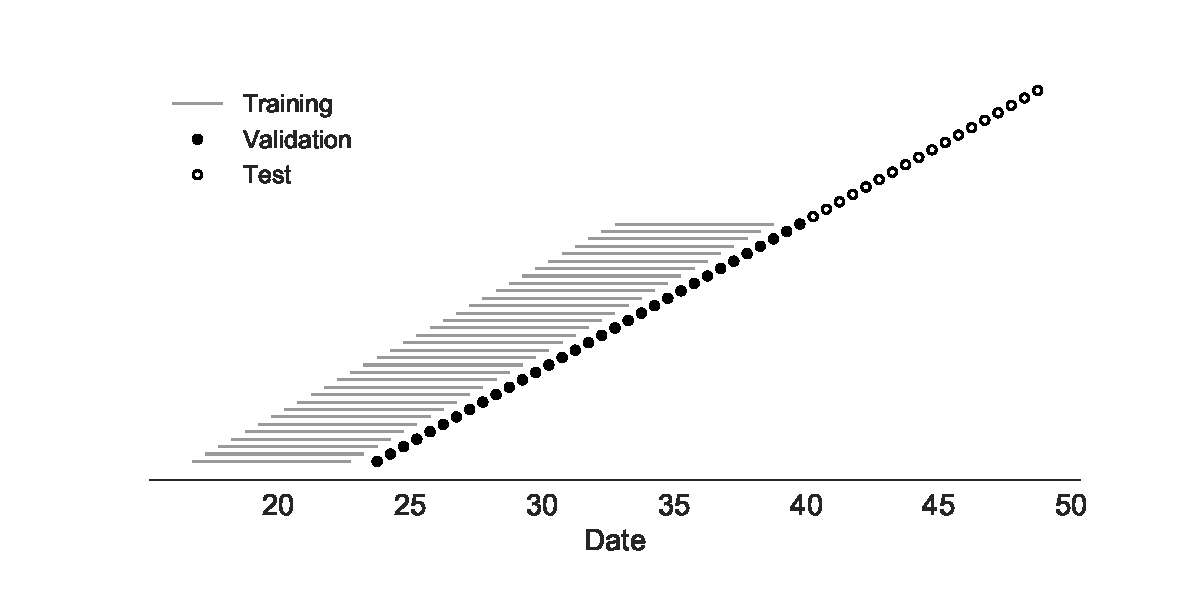
\includegraphics[width=\textwidth]{figures/cross-validation-for-simulated-populations.pdf}
  \caption{
  Time-series cross-validation scheme for simulated populations.
  Models were trained in six-year sliding windows (grey lines) and validated on out-of-sample data from validation timepoints (filled circles).
  Validation results from 30 years of data were used to iteratively tune model hyperparameters.
  After fixing hyperparameters, model coefficients were fixed at the mean values across all training windows.
  Fixed coefficients were applied to 9 years of new out-of-sample test data (open circles) to estimate true forecast errors.
  }
  \label{sup_fig:cross_validation_for_simulated_populations}
  \end{center}
\end{figure}

\begin{figure}[H]
  \begin{center}
  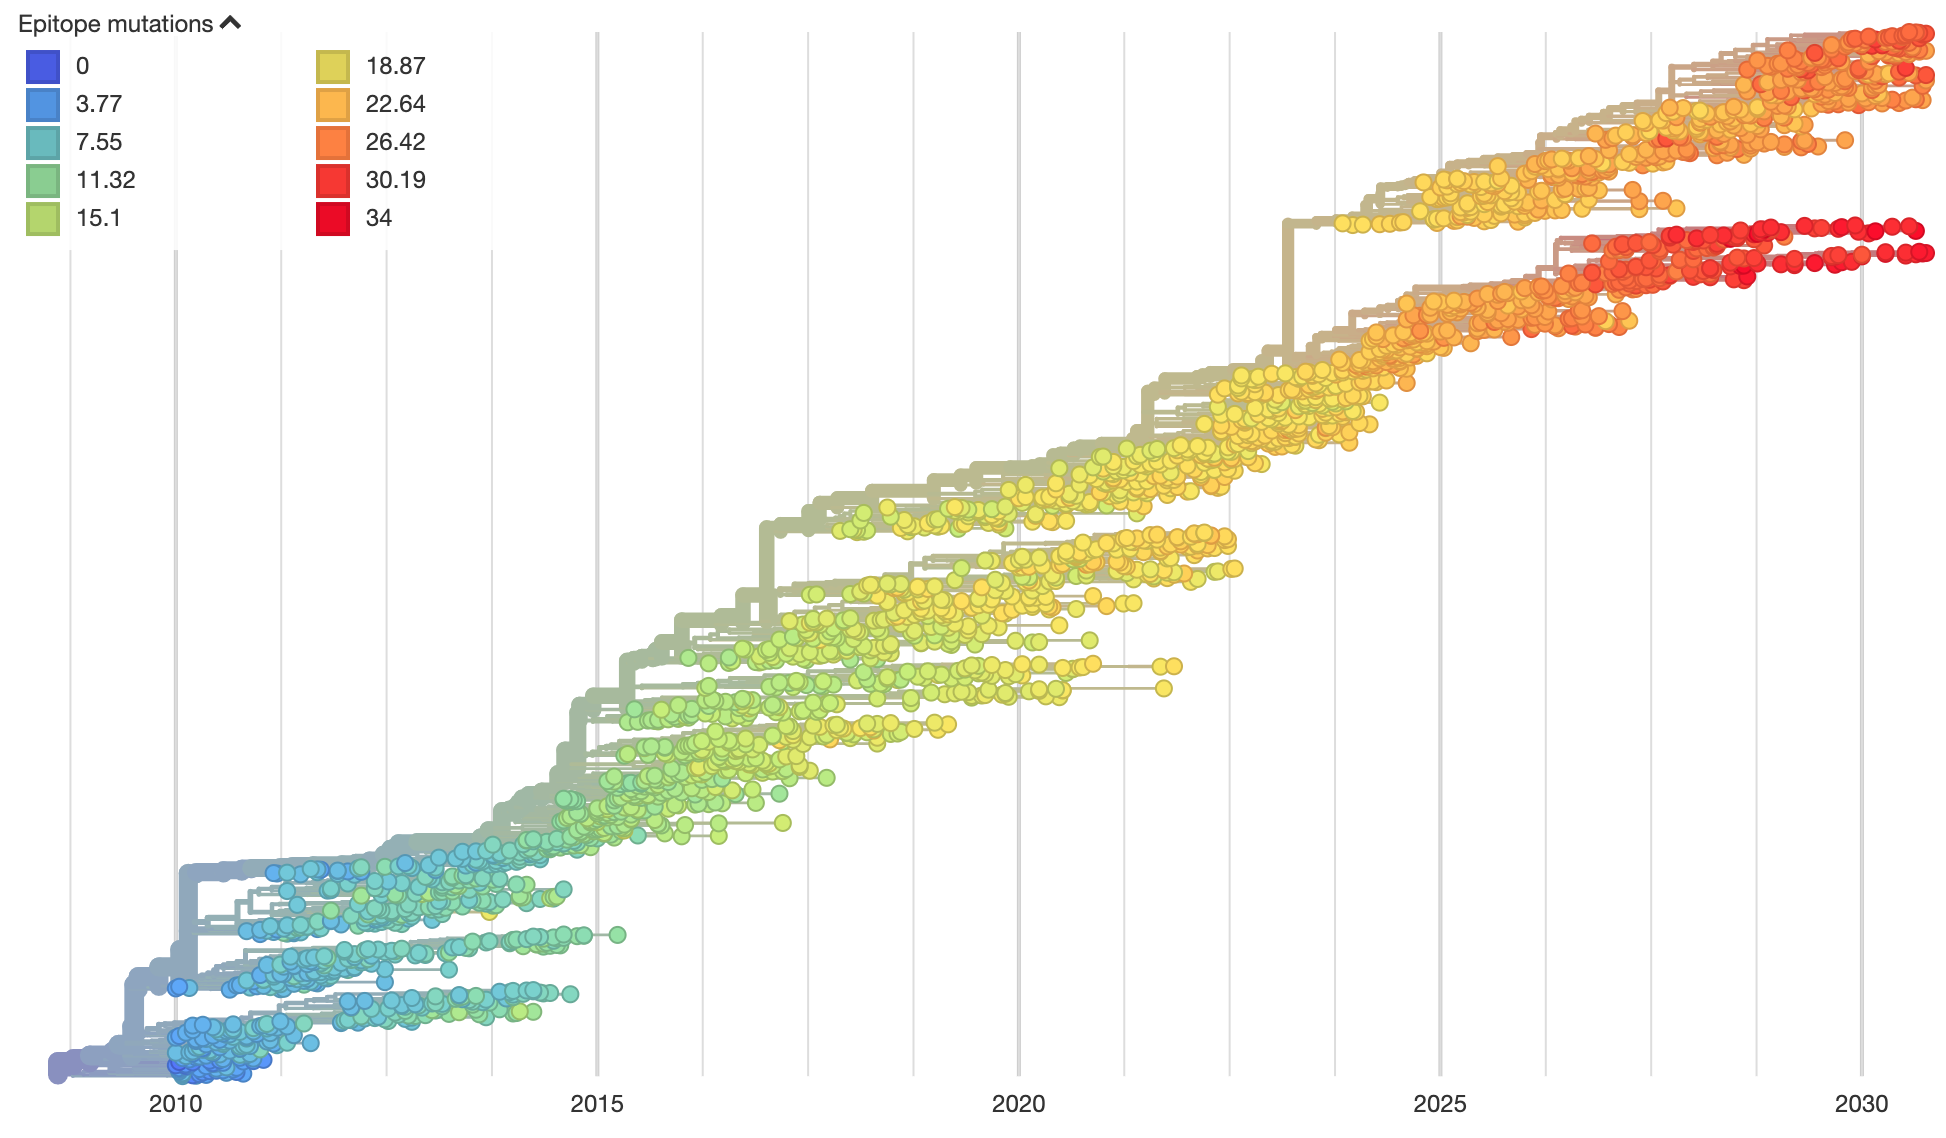
\includegraphics[width=\textwidth]{figures/simulated-h3n2-ha-phylogeny.png}
  \caption{
  Phylogeny of H3N2-like HA sequences sampled between the 24th and 30th years of simulated evolution.
  The phylogenetic structure and rate of accumulated epitope and non-epitope mutations match patterns observed in phylogenies of natural sequences.
  Sample dates were annotated as the generation in the simulation divided by 200 and added to 2000, to acquire realistic date ranges that were compatible with our modeling machinery.
  }
  \label{sup_fig:simulated_h3n2_ha_phylogeny}
  \end{center}
\end{figure}

\begin{figure}[H]
  \begin{center}
  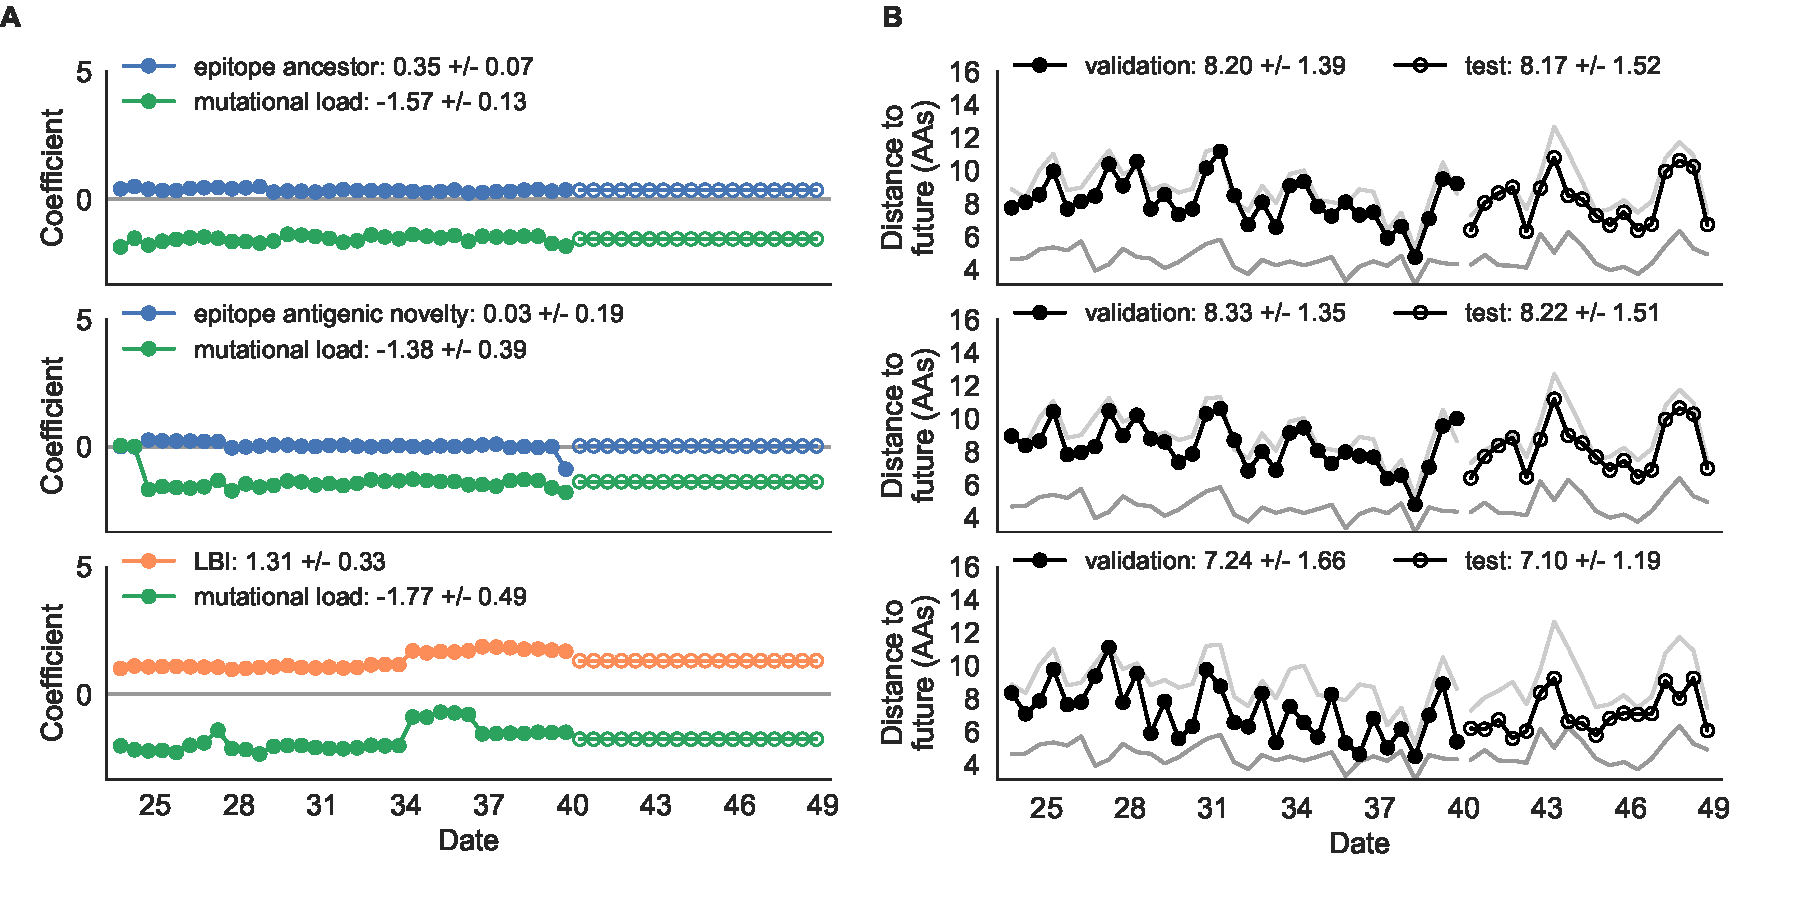
\includegraphics[width=\textwidth]{figures/unadjusted-composite-model-accuracy-and-coefficients-for-simulated-populations.pdf}
  \caption{
  Composite model coefficients and distances to the future for models fit to simulated populations.
  A) Coefficients and B) distances are shown per validation timepoint and test timepoint as in Fig.~\ref{fig:unadjusted_model_accuracy_and_coefficients_for_simulated_populations_controls}.
  }
  \label{sup_fig:unadjusted_composite_model_accuracy_and_coefficients_for_simulated_populations}
  \end{center}
\end{figure}

\begin{figure}[H]
  \begin{center}
  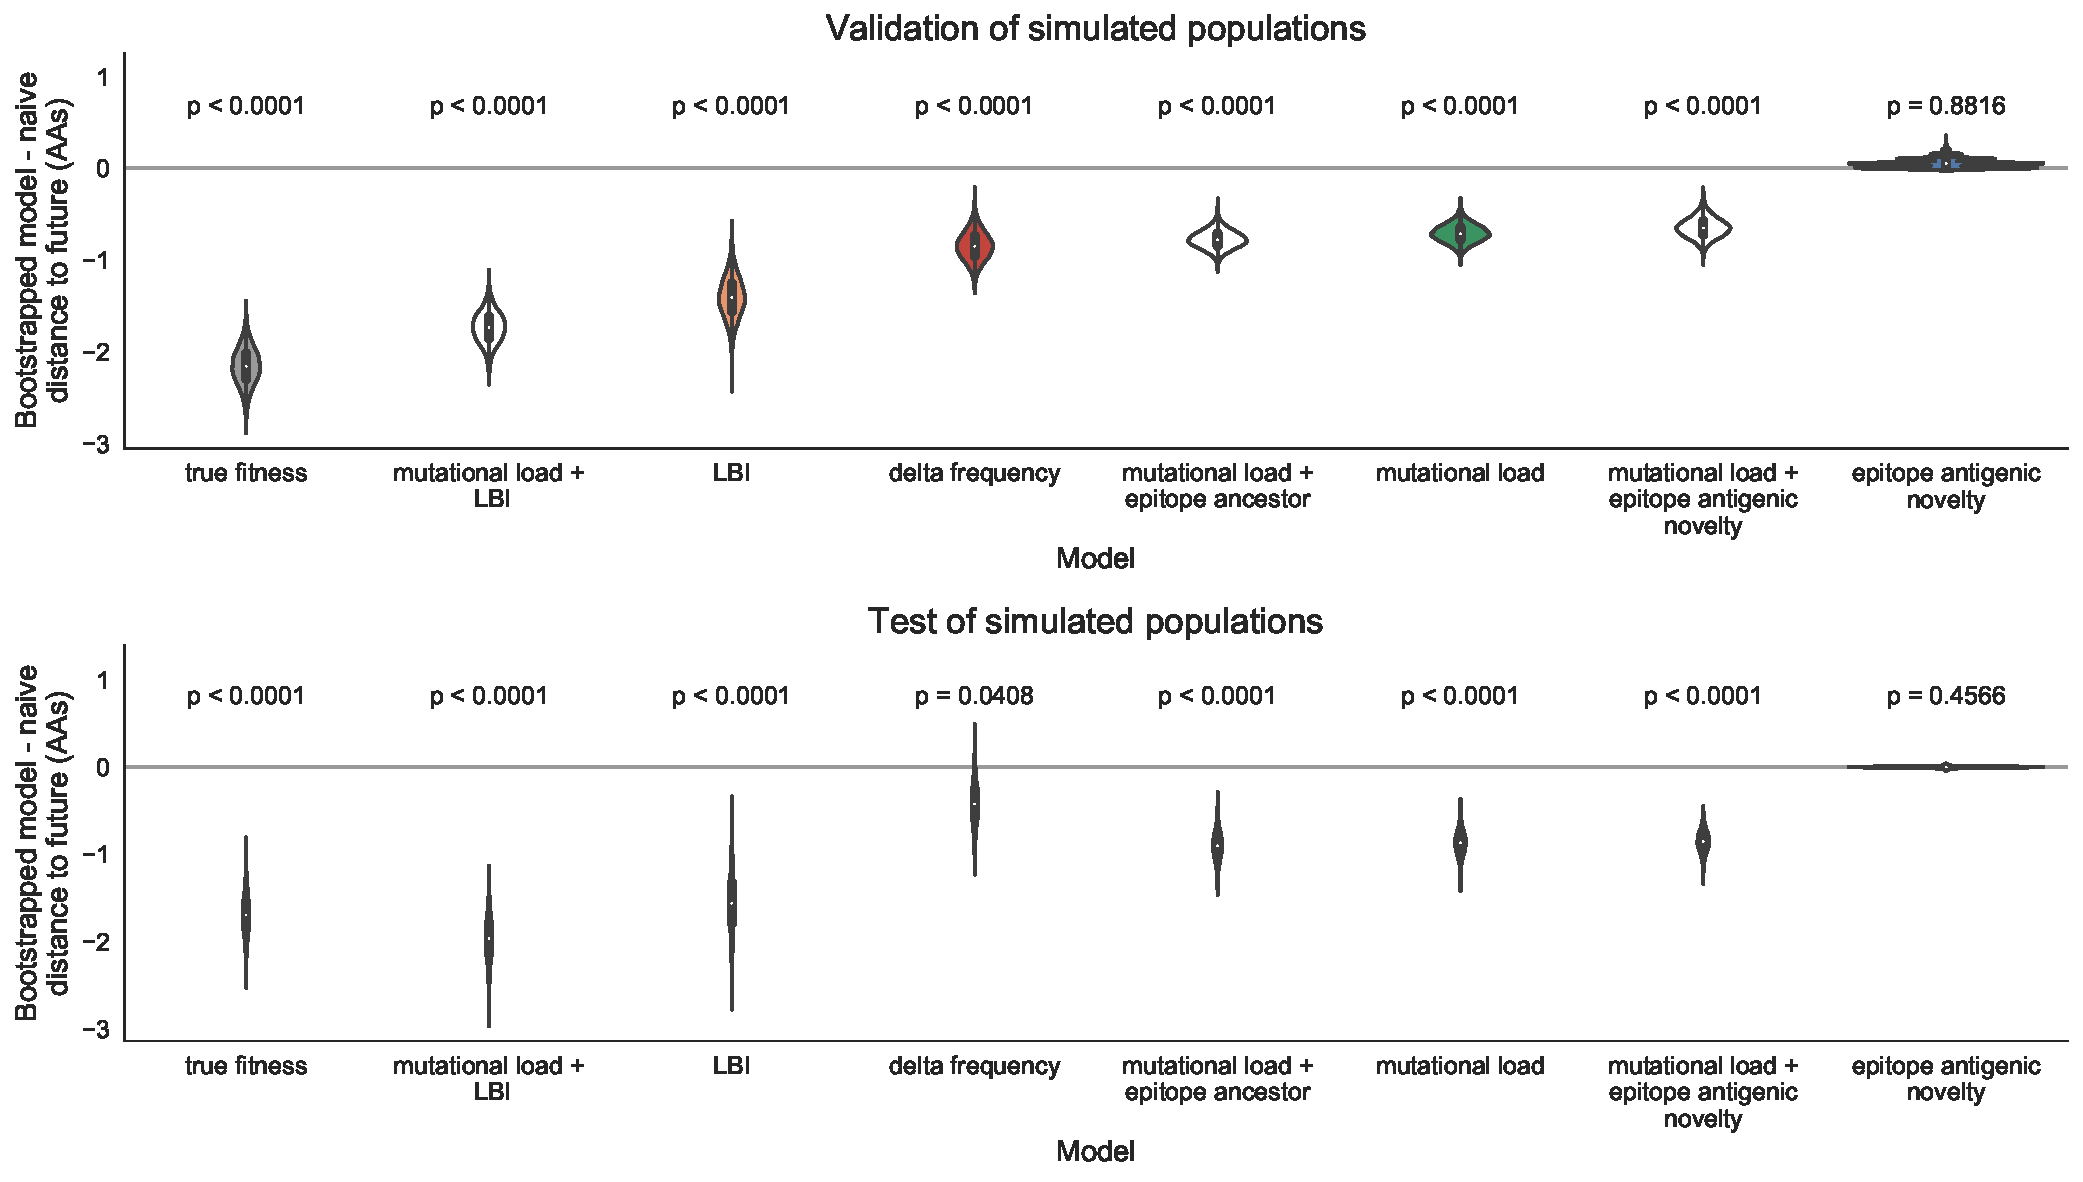
\includegraphics[width=\textwidth]{figures/bootstrap_distributions_for_simulated_sample_3.pdf}
  \caption{
  Bootstrap distributions of the mean difference of distances to the future between biologically-informed and naive models for simulated populations.
  Empirical differences in distances to the future were sampled with replacement and mean values for each bootstrap sample were calculated across n=10,000 bootstrap iterations.
  The horizontal gray line indicates a difference of zero between a given model and its corresponding naive model.
  Each model is annotated by the p-value representing the proportion of bootstrap samples with values less than zero (see Methods).
  }
  \label{sup_fig:bootstrap_distributions_for_simulated_sample_3}
  \end{center}
\end{figure}

\begin{figure}[H]
  \begin{center}
  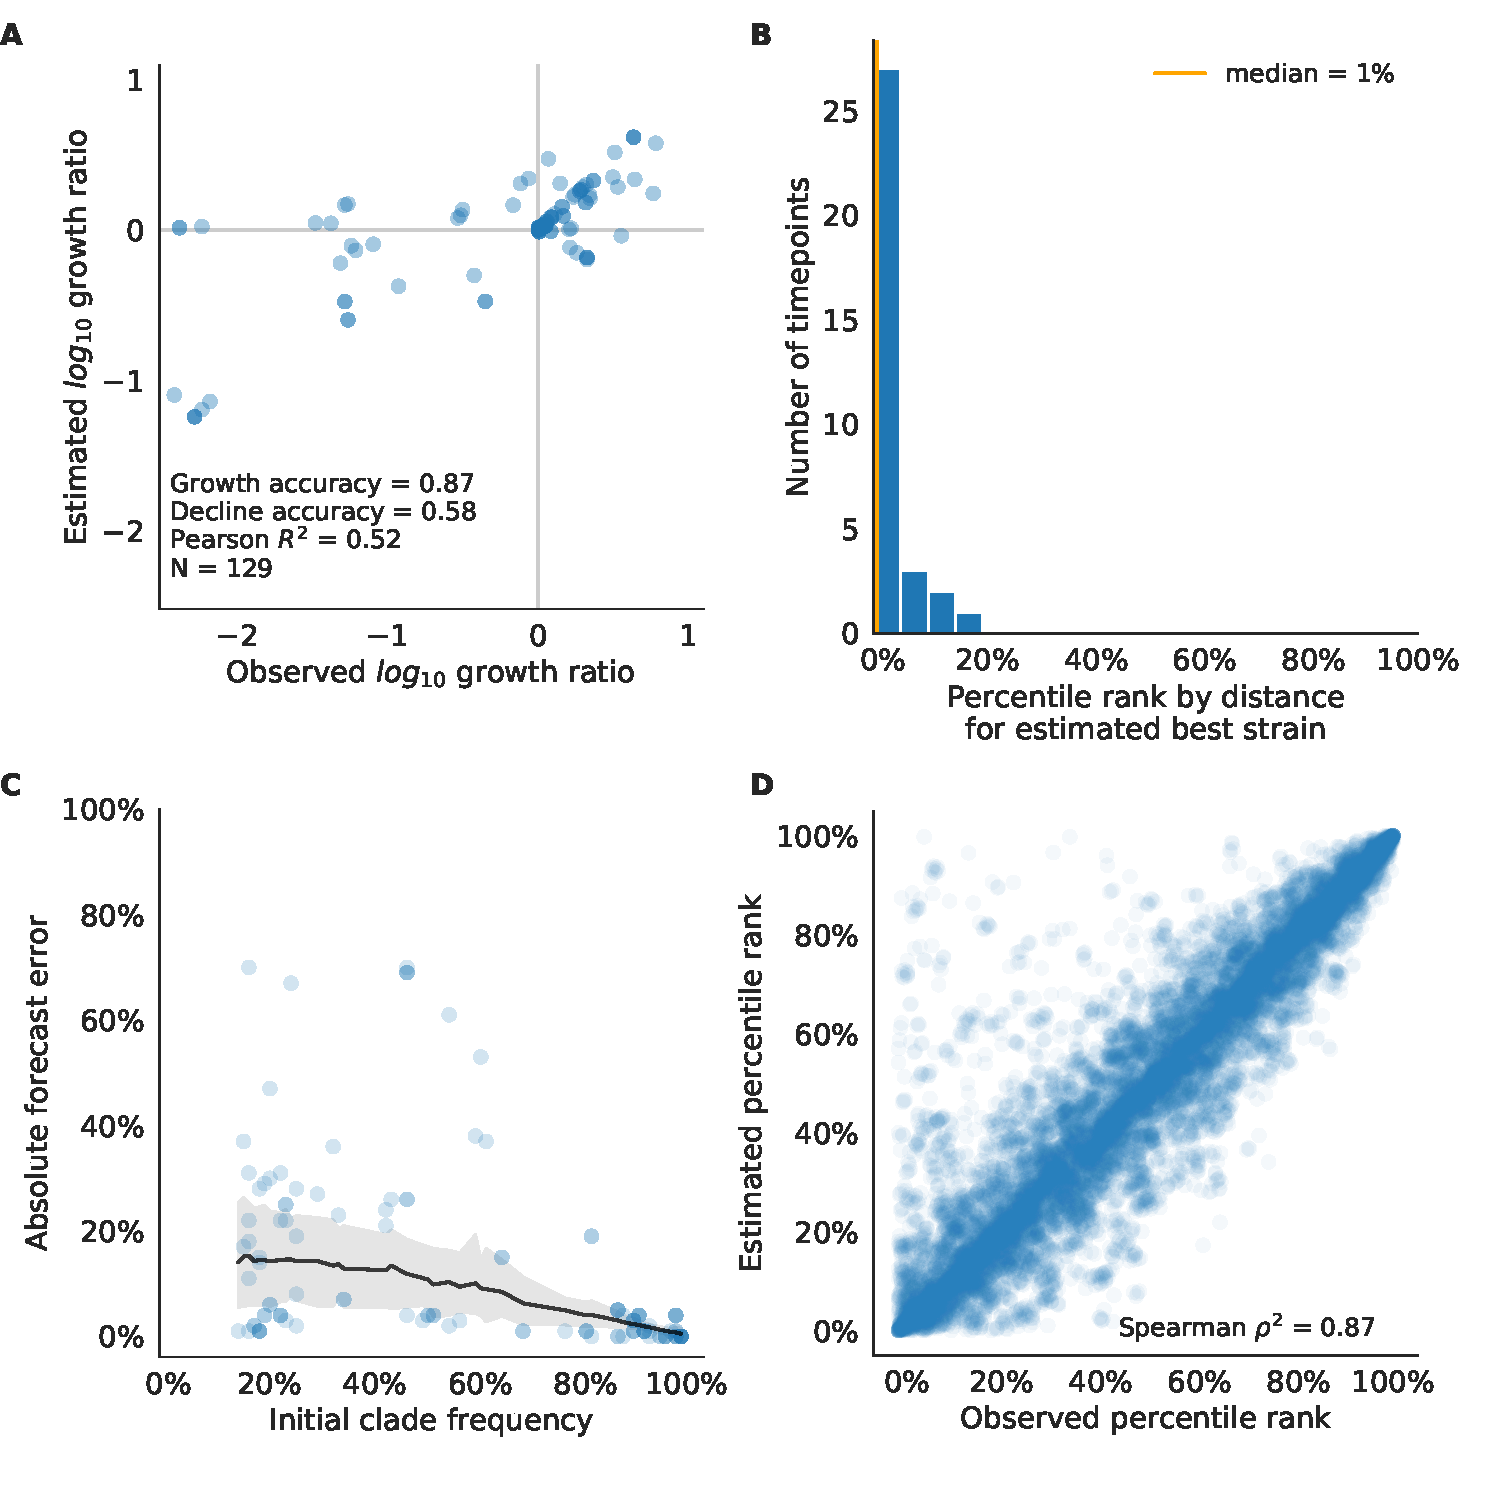
\includegraphics[width=\textwidth]{figures/validation-of-best-model-for-simulated-populations.pdf}
  \caption{
  Validation of best model for simulated populations of H3N2-like viruses.
  A) The correlation of estimated and observed clade frequency fold changes shows the model's ability to capture clade-level dynamics without explicitly optimizing for clade frequency targets.
  B) The rank of the estimated best strain based on its distance to the future for 33 timepoints.
  The estimated best strain was in the top 20th percentile of observed closest strains for 100\% of timepoints, confirming that the model makes a good choice when forced to select a single representative strain for the future population.
  C) Absolute forecast error for clades shown in A by their initial frequency with a mean LOESS fit (solid black line) and 95\% confidence intervals (grey shading) based on 100 bootstraps.
  D) The correlation of all strains at all timepoints by the percentile rank of their observed and estimated distances to the future.
  }
  \label{sup_fig:validation_of_best_model_for_simulated_populations}
  \end{center}
\end{figure}

\begin{figure}[H]
  \begin{center}
  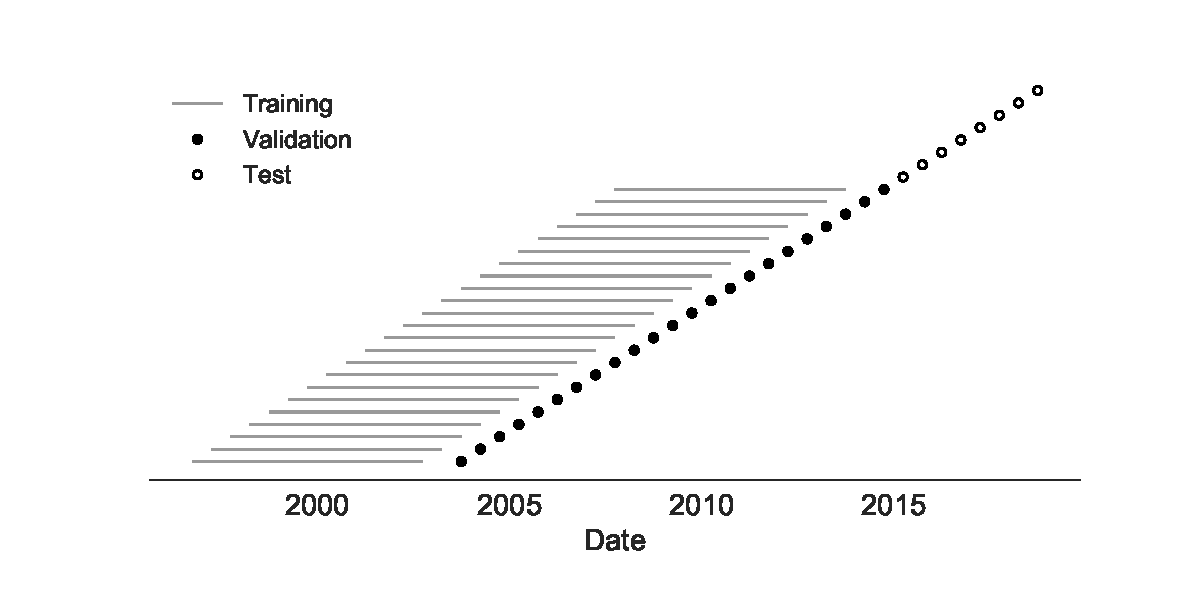
\includegraphics[width=\textwidth]{figures/cross-validation-for-natural-populations.pdf}
  \caption{
  Time-series cross-validation scheme for natural populations.
  Models were trained in six-year sliding windows (grey lines) and validated on out-of-sample data from validation timepoints (filled circles).
  Validation results from 25 years of data were used to iteratively tune model hyperparameters.
  After fixing hyperparameters, model coefficients were fixed at the mean values across all training windows.
  Fixed coefficients were applied to four years of new out-of-sample test data (open circles) to estimate true forecast errors.
  }
  \label{sup_fig:cross_validation_for_natural_populations}
  \end{center}
\end{figure}

\begin{figure}[H]
  \begin{center}
  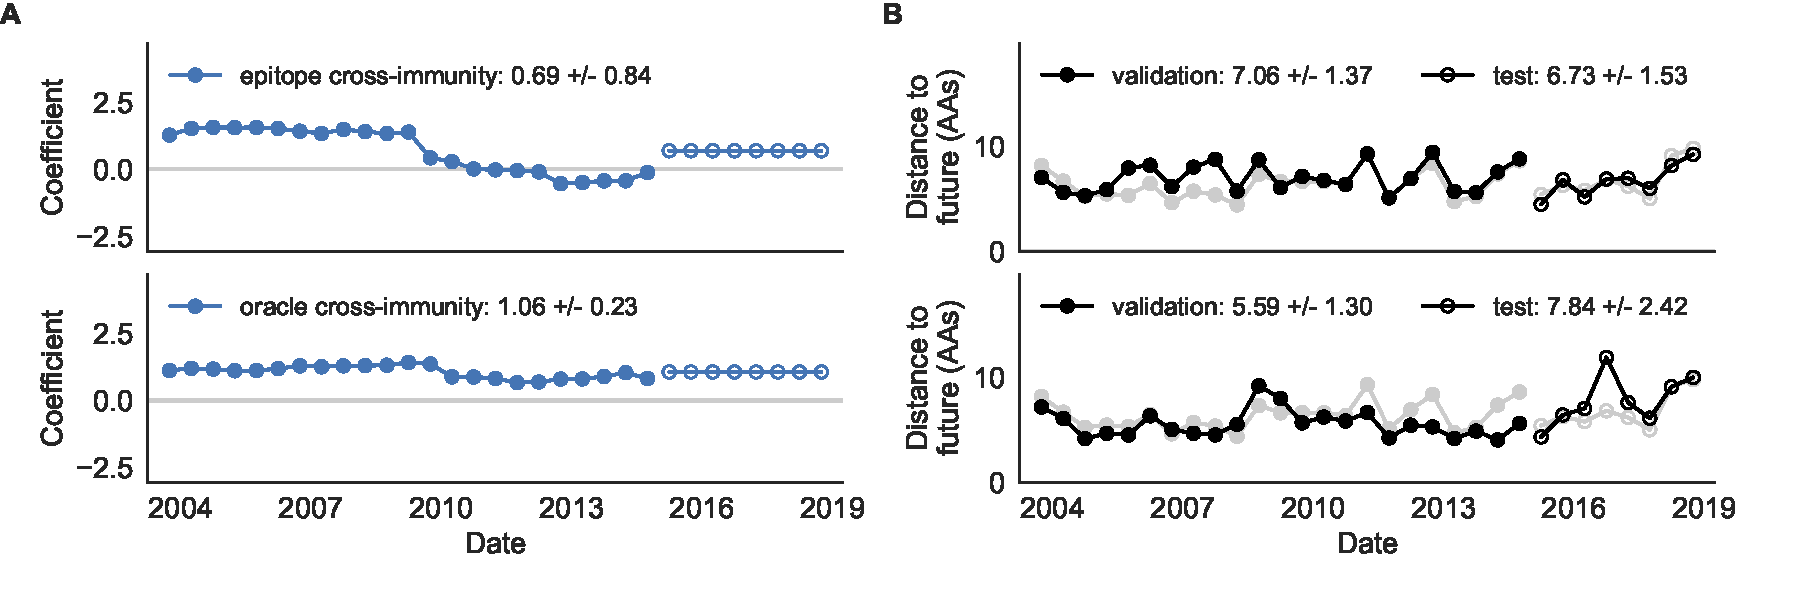
\includegraphics[width=\textwidth]{figures/unadjusted-composite-model-accuracy-and-coefficients-for-natural-populations-epitope-vs-oracle.pdf}
  \caption{
  Model coefficients and distances to the future for antigenic novelty models fit to natural populations.
  A) Coefficients and B) distances are shown per validation timepoint and test timepoint as in Fig.~\ref{fig:unadjusted_model_accuracy_and_coefficients_for_simulated_populations_controls}.
  The epitope antigenic novelty model relies on previously published epitope sites \cite{Luksza:2014hj}.
  The ``oracle'' antigenic novelty model relies on sites of beneficial mutations that were manually identified from the entire training and validation time period (Methods).
  The improved performance of the ``oracle'' model indicates that the sequence-based antigenic novelty metric can be effective when sites of beneficial mutations are known prior to forecasting.
  }
  \label{sup_fig:unadjusted_composite_model_accuracy_and_coefficients_for_natural_populations_epitope_vs_oracle}
  \end{center}
\end{figure}

\begin{figure}[H]
  \begin{center}
  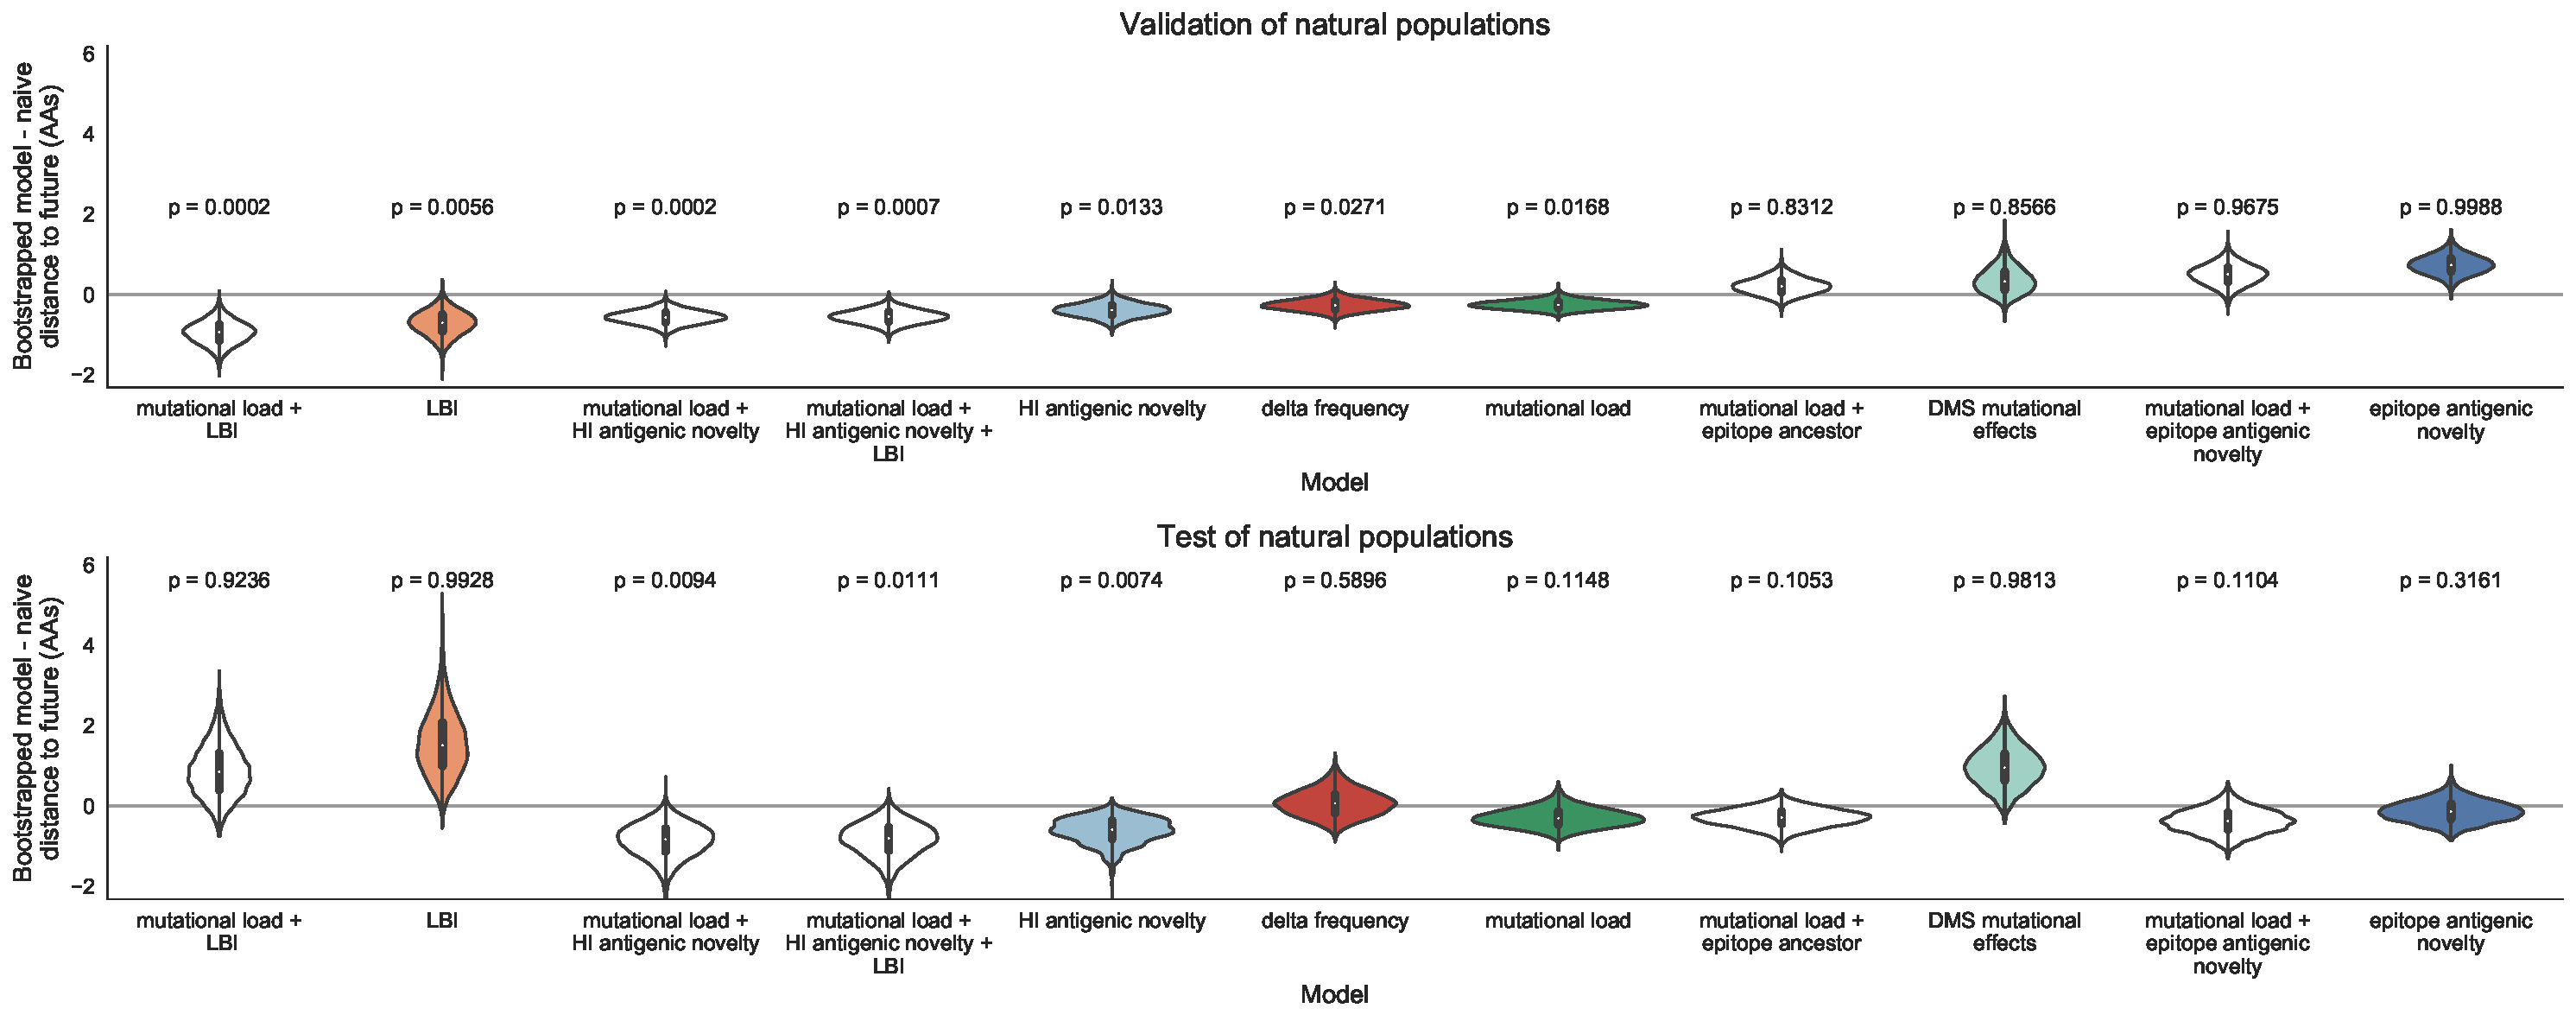
\includegraphics[width=\textwidth]{figures/bootstrap_distributions_for_natural_sample_1_with_90_vpm_sliding.pdf}
  \caption{
  Bootstrap distributions of the mean difference of distances to the future between biologically-informed and naive models for natural populations.
  Empirical differences in distances to the future were sampled with replacement and mean values for each bootstrap sample were calculated across n=10,000 bootstrap iterations.
  The horizontal gray line indicates a difference of zero between a given model and its corresponding naive model.
  Each model is annotated by the p-value representing the proportion of bootstrap samples with values less than zero (see Methods).
  }
  \label{sup_fig:bootstrap_distributions_for_natural_sample_1_with_90_vpm_sliding}
  \end{center}
\end{figure}

\begin{figure}[H]
  \begin{center}
  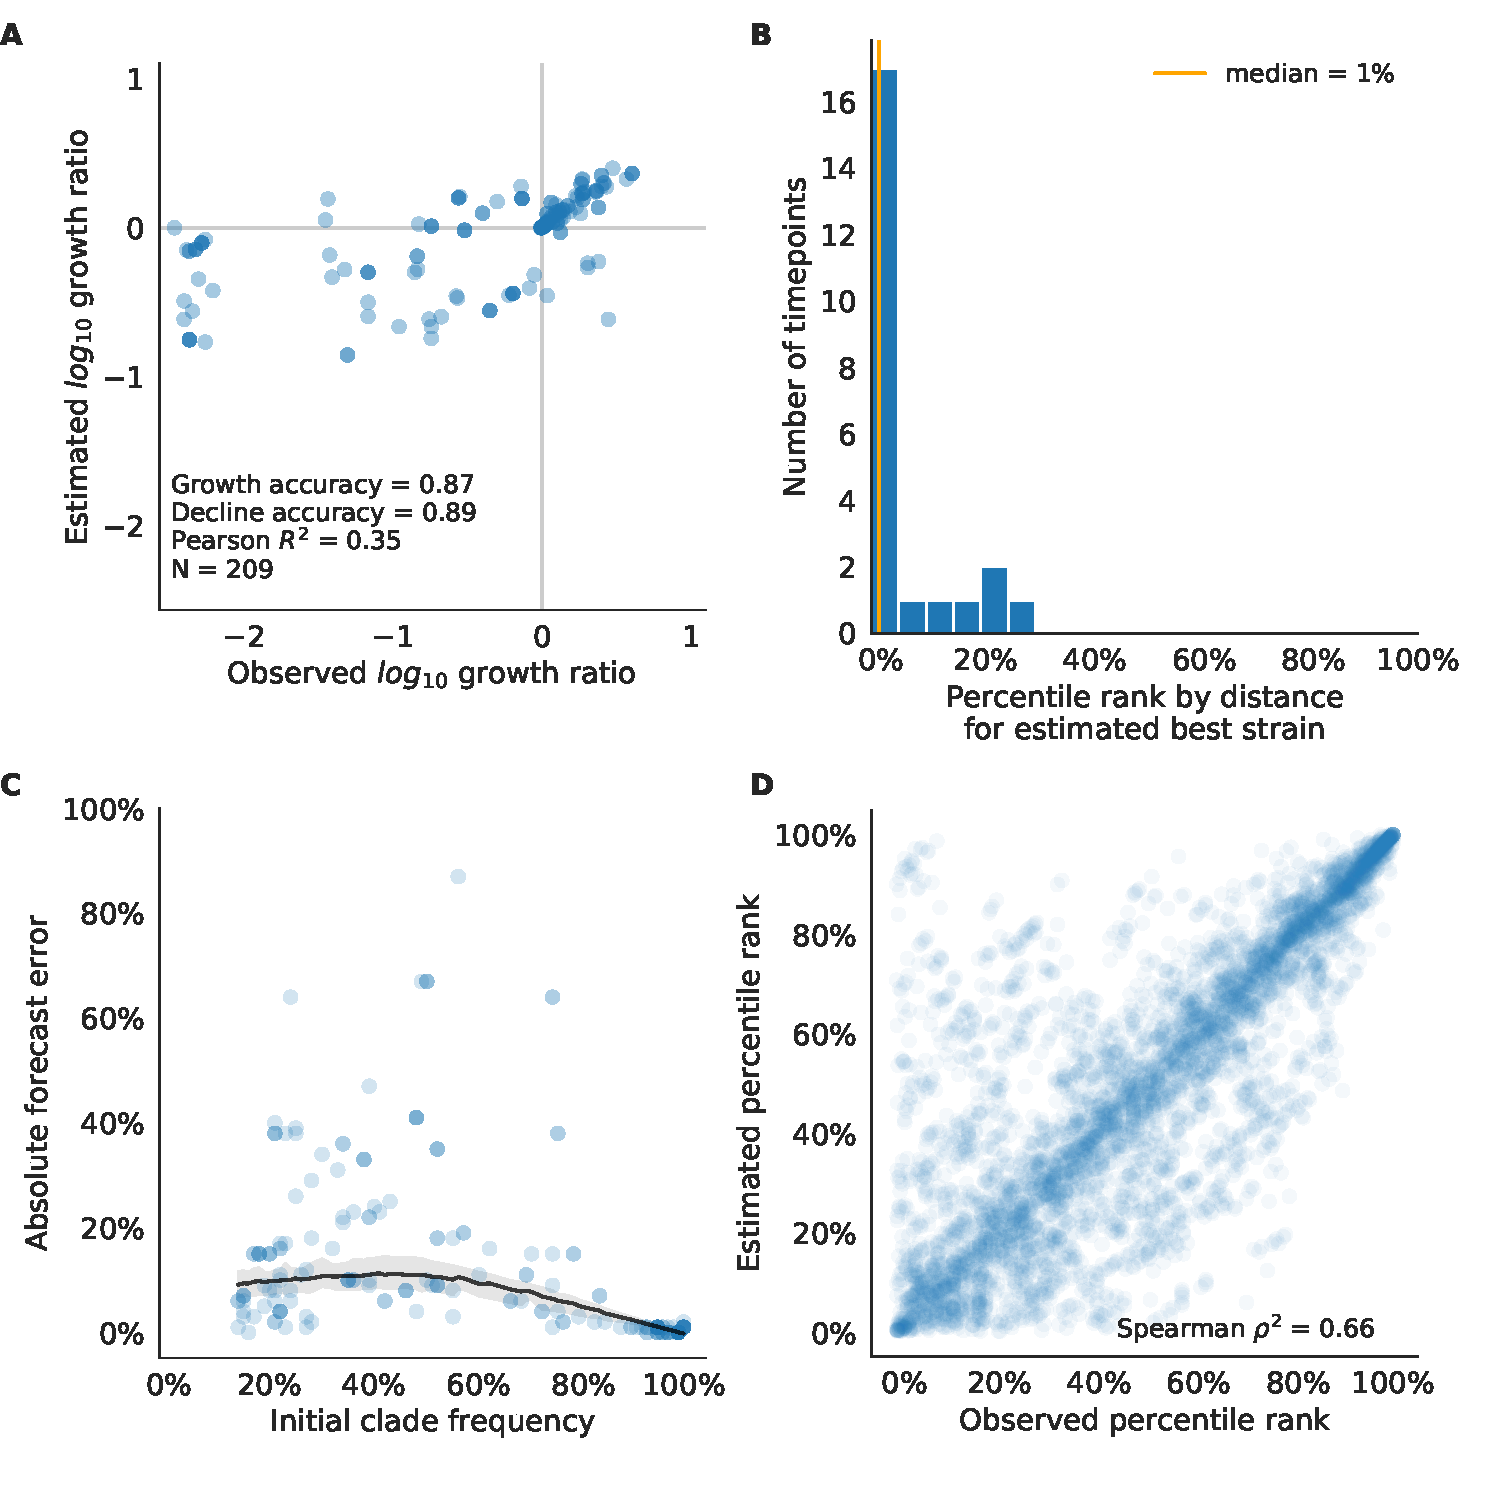
\includegraphics[width=\textwidth]{figures/validation-of-best-model-for-natural-populations.pdf}
  \caption{
  Validation of best model for natural populations of H3N2 viruses, the composite model of mutational load and LBI.
  A) The correlation of estimated and observed clade frequency fold changes shows the model's ability to capture clade-level dynamics without explicitly optimizing for clade frequency targets.
  B) The rank of the estimated best strain based on its distance to the future for 23 timepoints.
  The estimated best strain was in the top 20th percentile of observed closest strains for 87\% of timepoints, confirming that the model makes a good choice when forced to select a single representative strain for the future population.
  C) Absolute forecast error for clades shown in A by their initial frequency with a mean LOESS fit (solid black line) and 95\% confidence intervals (grey shading) based on 100 bootstraps.
  D) The correlation of all strains at all timepoints by the percentile rank of their observed and estimated distances to the future.
  }
  \label{sup_fig:validation_of_best_model_for_natural_populations}
  \end{center}
\end{figure}

\begin{figure}[H]
  \begin{center}
  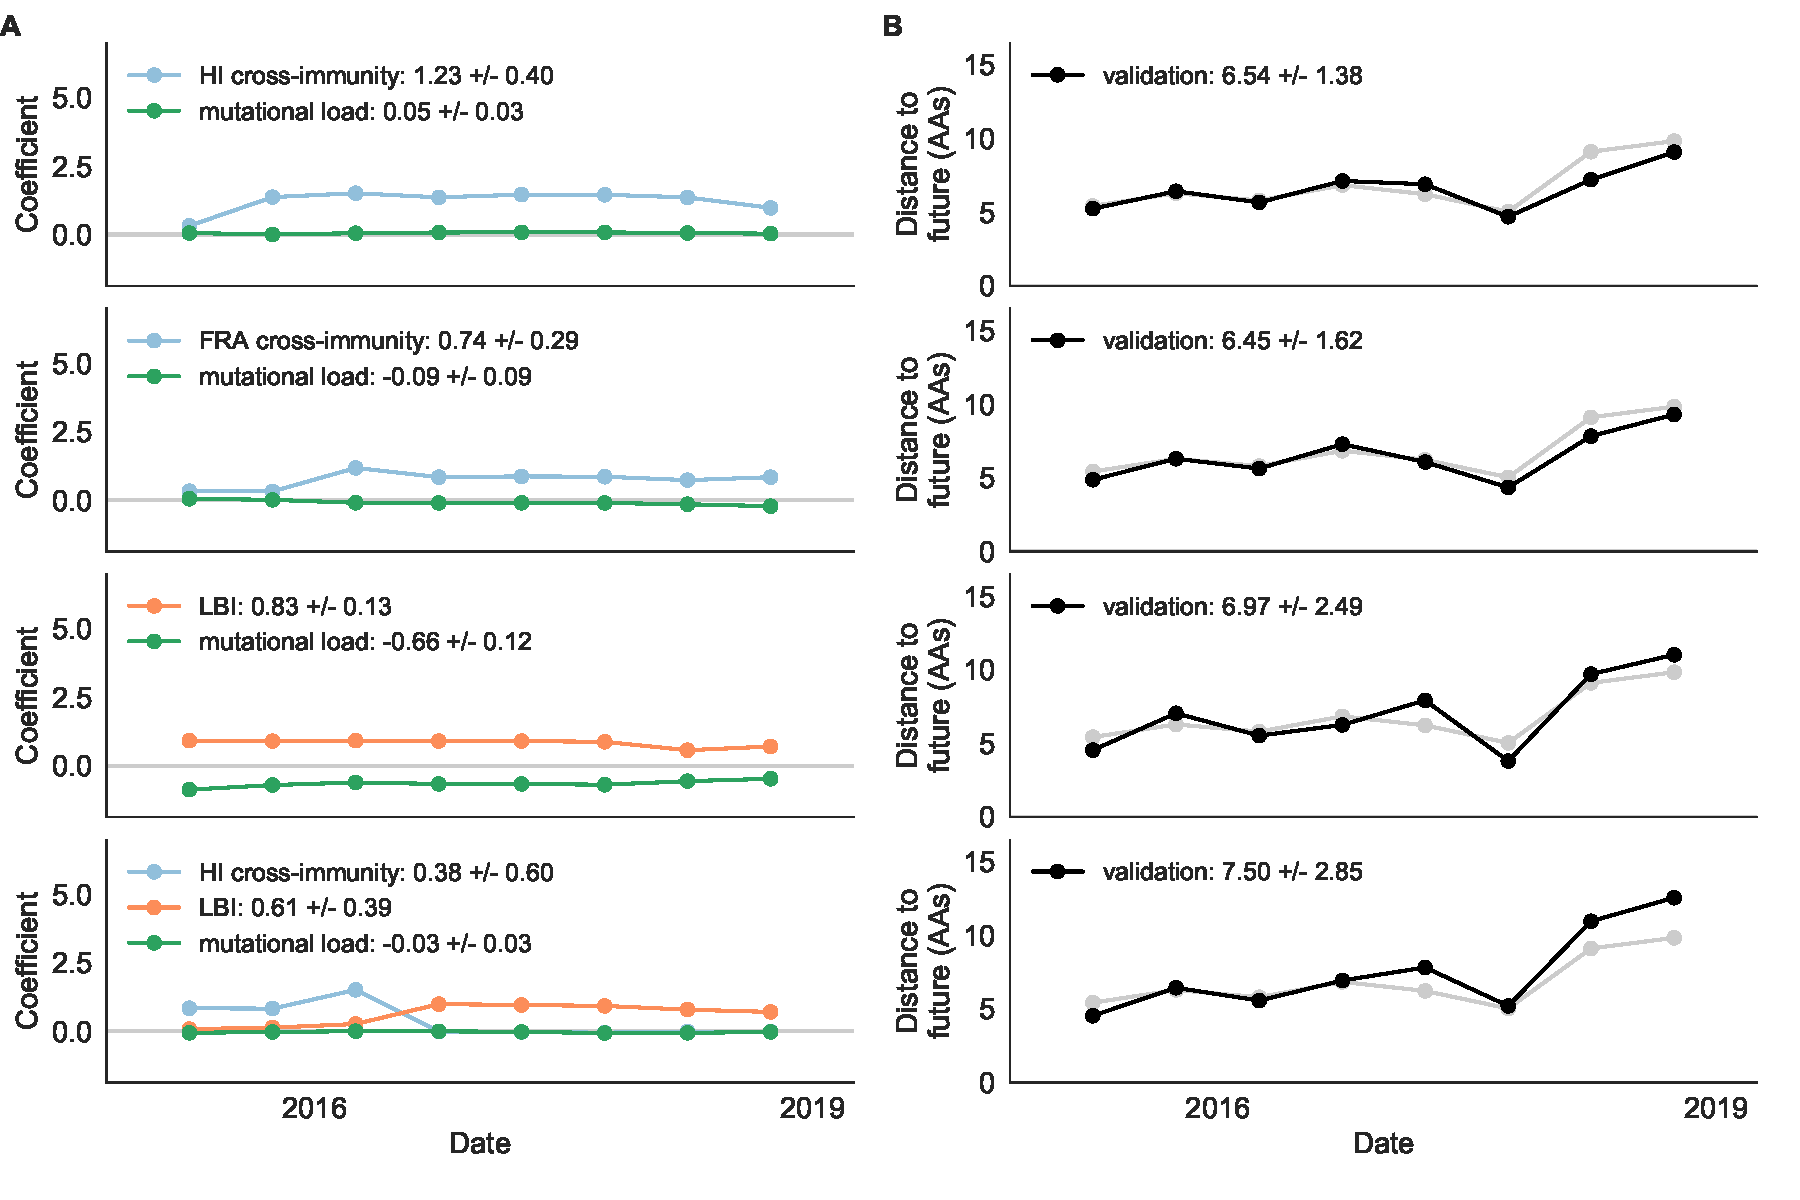
\includegraphics[width=\textwidth]{figures/models-natural-populations-composite-with-updated-coefficients-across-test-data.pdf}
  \caption{
    Model coefficients and distances to the future for best composite models and a FRA-based composite fit to recent data from natural populations as in Fig.~\ref{fig:unadjusted_model_accuracy_and_coefficients_for_simulated_populations_controls}.
    A) Coefficients and B) distances are shown per test timepoint (N=8).
    In contrast to the results for these models based on fixed coefficients from training/validation, these coefficients were learned for each six-year window prior to the corresponding test timepoint.
    The corresponding distances reflect the model's performance with updated coefficients on what is effectively new validation data.
    The naive model's distance to the future was 6.82 $\pm$ 1.74 AAs for these timepoints.
  }
  \label{sup_fig:updated_model_accuracy_and_coefficients_for_natural_populations_across_test_data}
  \end{center}
\end{figure}

\subsection*{Supplemental Tables}

\begin{table}[H]
  \begin{center}
    \begin{tabular}{lrrr}
\toprule
{} &  epitope mutations &  non-epitope mutations &  epitope-to-non-epitope ratio \\
branch type &                    &                        &                               \\
\midrule
side branch &                590 &                   1327 &                          0.44 \\
trunk       &                 23 &                     12 &                          1.92 \\
\bottomrule
\end{tabular}

    \caption{
    Number of epitope and non-epitope mutations per branch by trunk or side branch status for simulated populations.
    Epitope sites were defined previously described \cite{Luksza:2014hj}.
    Annotation of trunk and side branch was performed as previously described \cite{Bedford:2015fj}.
    Mutations were calculated for the full validation tree for simulated sequences samples between October of years 10 and 40.
    }
    \label{sup_table:mutations_by_trunk_status_for_simulated_populations}
  \end{center}
\end{table}

\begin{table}[H]
  \begin{center}
    \begin{tabular}{lrrr}
\toprule
{} &  epitope mutations &  non-epitope mutations &  epitope-to-non-epitope ratio \\
branch type &                    &                        &                               \\
\midrule
side branch &                485 &                   1177 &                          0.41 \\
trunk       &                 50 &                     32 &                          1.56 \\
\bottomrule
\end{tabular}

    \caption{
    Number of epitope and non-epitope mutations per branch by trunk or side branch status for natural populations.
    Epitope sites were defined previously described \cite{Luksza:2014hj}.
    Annotation of trunk and side branch was performed as previously described \cite{Bedford:2015fj}.
    Mutations were calculated for the full validation tree for natural sequences samples between 1990 and 2015.
    }
    \label{sup_table:mutations_by_trunk_status}
  \end{center}
\end{table}

\begin{table}[H]
  \begin{center}
    \scalebox{0.9}{
        \begin{tabular}{lll}
\toprule
                                           Model & \makecell{Distance closer \\ to future (AAs)} & \makecell{Model $>$ naive \\ (N=23)} \\
\midrule
                     non-epitope mutations + LBI &                                 0.96 +/- 1.42 &                            18 (78\%) \\
                                             LBI &                                 0.72 +/- 1.51 &                            17 (74\%) \\
       HI cross-immunity + non-epitope mutations &                                 0.63 +/- 0.79 &                            18 (78\%) \\
 HI cross-immunity + non-epitope mutations + LBI &                                 0.52 +/- 0.83 &                            19 (83\%) \\
                                         HI tree &                                 0.40 +/- 0.82 &                            15 (65\%) \\
                               HI cross-immunity &                                 0.36 +/- 0.65 &                            17 (74\%) \\
                                 delta frequency &                                 0.27 +/- 0.67 &                            16 (70\%) \\
                           non-epitope mutations &                                 0.26 +/- 0.56 &                            17 (74\%) \\
                          Koel epitope mutations &                                 0.19 +/- 0.25 &                            19 (83\%) \\
                                     DMS entropy &                                 0.02 +/- 0.15 &                            14 (61\%) \\
                                 DMS non-epitope &                                -0.05 +/- 0.15 &                             7 (30\%) \\
                        linear HI mut phenotypes &                                -0.06 +/- 0.51 &                            11 (48\%) \\
                           HI sub cross-immunity &                                -0.14 +/- 0.57 &                            10 (43\%) \\
                          Wolf epitope mutations &                                -0.17 +/- 0.31 &                             5 (22\%) \\
                          DMS mutational effects &                                -0.35 +/- 1.65 &                            11 (48\%) \\
                               epitope mutations &                                -0.43 +/- 0.94 &                             5 (22\%) \\
  epitope cross-immunity + non-epitope mutations &                                -0.54 +/- 1.39 &                             6 (26\%) \\
                          epitope cross-immunity &                                -0.66 +/- 1.13 &                             6 (26\%) \\
\bottomrule
\end{tabular}

    }
    \caption{
      All model coefficients and performance on validation and test data for natural populations ordered from best to worst by distance to the future, as in Table~\ref{table_simulated_model_selection}.
      Distances annotated with asterisks (*) were significantly closer to the future than the naive model as measured by bootstrap tests (see Methods and Supplemental Fig.~\ref{sup_fig:bootstrap_distributions_for_natural_sample_1_with_90_vpm_sliding}).
      Validation results are based on 23 timepoints.
      Test results are based on eight timepoints not observed during model training and validation.
      Model results for additional variants of fitness metrics including those based on epitope mutations and DMS preferences are included for reference.
    }
    \label{sup_table:complete_natural_model_selection}
  \end{center}
\end{table}

\begin{table}[H]
  \begin{center}
    \scalebox{0.8}{
        \begin{tabular}{llllrrl}
\toprule
    sample &  error\_type &      individual\_model &                         composite\_model &  bootstrap\_mean &  bootstrap\_std &    p\_value \\
\midrule
 simulated &  validation &          true fitness &                  mutational load +  LBI &            0.43 &           0.23 &     0.9667 \\
 simulated &  validation &       mutational load &                  mutational load +  LBI &           -1.03 &           0.21 &  $<$0.0001 \\
 simulated &  validation &                   LBI &                  mutational load +  LBI &           -0.33 &           0.14 &     0.0096 \\
 simulated &        test &          true fitness &                  mutational load +  LBI &           -0.28 &           0.26 &     0.1396 \\
 simulated &        test &       mutational load &                  mutational load +  LBI &           -1.11 &           0.25 &  $<$0.0001 \\
 simulated &        test &                   LBI &                  mutational load +  LBI &           -0.41 &           0.16 &     0.0001 \\
   natural &  validation &       mutational load &                  mutational load +  LBI &           -0.69 &           0.27 &     0.0028 \\
   natural &  validation &                   LBI &                  mutational load +  LBI &           -0.23 &           0.10 &     0.0028 \\
   natural &  validation &       mutational load &  mutational load + HI antigenic novelty &           -0.31 &           0.18 &     0.0409 \\
   natural &  validation &  HI antigenic novelty &  mutational load + HI antigenic novelty &           -0.18 &           0.11 &     0.0586 \\
   natural &        test &       mutational load &                  mutational load +  LBI &            1.18 &           0.80 &     0.9406 \\
   natural &        test &                   LBI &                  mutational load +  LBI &           -0.69 &           0.24 &  $<$0.0001 \\
   natural &        test &       mutational load &  mutational load + HI antigenic novelty &           -0.57 &           0.32 &     0.0123 \\
   natural &        test &  HI antigenic novelty &  mutational load + HI antigenic novelty &           -0.24 &           0.18 &     0.0976 \\
\bottomrule
\end{tabular}

    }
    \caption{
      Comparison of composite and individual model distances to the future by bootstrap test (see Methods).
      Empirical differences represent the mean difference between the composite and individual models' distances to the future at each timepoint.
      The p values represent the proportion of n=10,000 bootstrap samples where the mean difference was greater than or equal to zero.
    }
    \label{sup_table:composite_vs_individual_model_comparison}
  \end{center}
\end{table}

\pagebreak

\subsection*{Supplemental Text}

\subsubsection*{GISAID Acknowledgements}

WHO Collaborating Centre for Reference and Research on Influenza, Victorian Infectious Diseases Reference Laboratory, Australia; WHO Collaborating Centre for Reference and Research on Influenza, Chinese National Influenza Center, China; WHO Collaborating Centre for Reference and Research on Influenza, National Institute of Infectious Diseases, Japan; The Crick Worldwide Influenza Centre, The Francis Crick Institute, United Kingdom; WHO Collaborating Centre for the Surveillance, Epidemiology and Control of Influenza, Centers for Disease Control and Prevention, United States; ADImmune Corporation, Taiwan; ADPH Bureau of Clinical Laboratories, United States; Aichi Prefectural Institute of Public Health, Japan; Akershus University Hospital, Norway; Akita Research Center for Public Health and Environment, Japan; Alabama State Laboratory, United States; Alaska State Public Health Laboratory, United States; Alaska State Virology Lab, United States; Aomori Prefectural Institute of Public Health and Environment, Japan; Aristotelian University of Thessaloniki, Greece; Arizona Department of Health Services, United States; Arkansas Children's Hospital, United States; Arkansas Department of Health, United States; Auckland Healthcare, New Zealand; Auckland Hospital, New Zealand; Austin Health, Australia; Baylor College of Medicine, United States; California Department of Health Services, United States; Canberra Hospital, Australia; Cantacuzino Institute, Romania; Canterbury Health Services, New Zealand; Caribbean Epidemiology Center, Trinidad and Tobago; CDC GAP Nigeria, Nigeria; CDC-Kenya, Kenya; CEMIC University Hospital, Argentina; CENETROP, Bolivia, Plurinationial State of; Center for Disease Control, Taiwan; Center for Public Health and Environment, Hiroshima Prefectural Technology Research Institute, Japan; Central Health Laboratory, Mauritius; Central Laboratory of Public Health, Paraguay; Central Public Health Laboratory, Ministry of Health, Oman; Central Public Health Laboratory, Palestinian Territory; Central Public Health Laboratory, Papua New Guinea; Central Research Institute for Epidemiology, Russian Federation; Centre for Diseases Control and Prevention, Armenia; Centre for Infections, Health Protection Agency, United Kingdom; Centre Pasteur du Cameroun, Cameroon; Chiba City Institute of Health and Environment, Japan; Chiba Prefectural Institute of Public Health, Japan; Childrens Hospital Westmead, Australia; Chuuk State Hospital, Micronesia, Federated States of; City of El Paso Dept of Public Health, United States; Clinical Virology Unit, CDIM, Australia; Colorado Department of Health Lab, United States; Connecticut Department. of Public Health, United States; Contiguo a Hospital Rosales, El Salvador; Croatian Institute of Public Health , Croatia; CRR virus Influenza region Sud, France; CRR virus Influenza region Sud, Guyana; CSL Ltd, United States; Dallas County Health and Human Services, United States; DC Public Health Lab, United States; Delaware Public Health Lab, United States; Departamento de Laboratorio de Salud Publica, Uruguay; Department of Virology, Medical University Vienna, Austria; Disease Investigation Centre Wates (BBVW), Australia; Drammen Hospital / Vestreviken HF, Norway; Ehime Prefecture Institute of Public Health and Environmental Science, Japan; Erasmus Medical Center, Netherlands; Erasmus University of Rotterdam, Netherlands; Ethiopian Health and Nutrition Research Institute (EHNRI), Ethiopia; Evanston Hospital and NorthShore University, United States; Facultad de Medicina, Spain; Fiji Centre for Communicable Disease Control, Fiji; Florida Department of Health, United States; Fukui Prefectural Institute of Public Health, Japan; Fukuoka City Institute for Hygiene and the Environment, Japan; Fukuoka Institute of Public Health and Environmental Sciences, Japan; Fukushima Prefectural Institute of Public Health, Japan; Gart Naval General Hospital, United Kingdom; Georgia Public Health Laboratory, United States; Gifu Municipal Institute of Public Health, Japan; Gifu Prefectural Institute of Health and Environmental Sciences, Japan; Government Virus Unit, Hong Kong; Gunma Prefectural Institute of Public Health and Environmental Sciences, Japan; Hamamatsu City Health Environment Research Center, Japan; Haukeland University Hospital, Dept. of Microbiology , Norway; Headquarters British Gurkhas Nepal, Nepal; Health Forde, Department of Microbiology, Norway; Health Protection Agency, United Kingdom; Health Protection Inspectorate, Estonia; Hellenic Pasteur Institute, Greece; Hiroshima City Institute of Public Health, Japan; Hokkaido Institute of Public Health, Japan; Hopital Cantonal Universitaire de Geneves, Switzerland; Hopital Charles Nicolle, Tunisia; Hospital Clinic de Barcelona, Spain; Hospital Universitari Vall d'Hebron, Spain; Houston Department of Health and Human Services, United States; Hyogo Prefectural Institute of Public Health and Consumer Sciences, Japan; Ibaraki Prefectural Institute of Public Health, Japan; Illinois Department of Public Health, United States; Indiana State Department of Health Laboratories, United States; Infectology Center of Latvia, Latvia; Innlandet Hospital Trust, Division Lillehammer, Department for Microbiology, Norway; INSA National Institute of Health Portugal, Portugal; Institut National d'Hygiene, Morocco; Institut Pasteur d'Algerie, Algeria; Institut Pasteur de Dakar, Senegal; Institut Pasteur de Madagascar, Madagascar; Institut Pasteur in Cambodia, Cambodia; Institut Pasteur New Caledonia, New Caledonia; Institut Pasteur, France; Institut Pasteur, Saudi Arabia; Institut Penyelidikan Perubatan, Malaysia; Institute National D'Hygiene, Togo; Institute of Environmental Science and Research, New Zealand; Institute of Environmental Science and Research, Tonga; Institute of Epidemiology and Infectious Diseases, Ukraine; Institute of Epidemiology Disease Control and Research, Bangladesh; Institute of Immunology and Virology Torlak, Serbia; Institute of Medical and Veterinary Science (IMVS), Australia; Institute of Public Health, Serbia; Institute of Public Health, Albania; Institute of Public Health, Montenegro; Institute Pasteur du Cambodia, Cambodia; Instituto Adolfo Lutz, Brazil; Instituto Conmemorativo Gorgas de Estudios de la Salud, Panama; Instituto de Salud Carlos III, Spain; Instituto de Salud Publica de Chile, Chile; Instituto Nacional de Enfermedades Infecciosas, Argentina; Instituto Nacional de Higiene Rafael Rangel, Venezuela, Bolivia; Instituto Nacional de Laboratoriosde Salud (INLASA), Bolivia; Instituto Nacional de Salud de Columbia, Colombia; Instituto Nacional de Saude, Portugal; Iowa State Hygienic Laboratory, United States; IRSS, Burkina Faso; Ishikawa Prefectural Institute of Public Health and Environmental Science, Japan; ISS, Italy; Istanbul University, Turkey; Istituto Superiore di Sanità, Italy; Ivanovsky Research Institute of Virology RAMS, Russian Federation; Jiangsu Provincial Center for Disease Control and Prevention, China; John Hunter Hospital, Australia; Kagawa Prefectural Research Institute for Environmental Sciences and Public Health, Japan; Kagoshima Prefectural Institute for Environmental Research and Public Health, Japan; Kanagawa Prefectural Institute of Public Health, Japan; Kansas Department of Health and Environment, United States; Kawasaki City Institute of Public Health , Japan; Kentucky Division of Laboratory Services, United States; Kitakyusyu City Institute of Enviromental Sciences, Japan; Kobe Institute of Health, Japan; Kochi Public Health and Sanitation Institute, Japan; Kumamoto City Environmental Research Center, Japan; Kumamoto Prefectural Institute of Public Health and Environmental Science, Japan; Kyoto City Institute of Health and Environmental Sciences, Japan; Kyoto Prefectural Institute of Public Health and Environment, Japan; Laboratoire National de Sante Publique, Haiti; Laboratoire National de Sante, Luxembourg; Laboratório Central do Estado do Paraná, Brazil; Laboratorio Central do Estado do Rio de Janeiro, Brazil; Laboratorio de Investigacion / Centro de Educacion Medica y Amistad Dominico Japones (CEMADOJA), Dominican Republic; Laboratorio De Saude Publico, Macao; Laboratorio de Virologia, Direccion de Microbiologia, Nicaragua; Laboratorio de Virus Respiratorio, Mexico; Laboratorio Nacional de Influenza, Costa Rica; Laboratorio Nacional De Salud Guatemala, Guatemala; Laboratorio Nacional de Virologia, Honduras; Laboratory Directorate, Jordan; Laboratory for Virology, National Institute of Public Health, Slovenia; Laboratory of Influenza and ILI, Belarus; LACEN/RS - Laboratório Central de Saúde Pública do Rio Grande do Sul, Brazil; Landspitali - University Hospital, Iceland; Lithuanian AIDS Center Laboratory, Lithuania; Los Angeles Quarantine Station, CDC Quarantine Epidemiology and Surveillance Team, United States; Louisiana Department of Health and Hospitals, United States; Maine Health and Environmental Testing Laboratory, United States; Malbran, Argentina; Marshfield Clinic Research Foundation, United States; Maryland Department of Health and Mental Hygiene, United States; Massachusetts Department of Public Health, United States; Mater Dei Hospital, Malta; Medical Research Institute, Sri Lanka; Medical University Vienna, Austria; Melbourne Pathology, Australia; Michigan Department of Community Health, United States; Mie Prefecture Health and Environment Research Institute, Japan; Mikrobiologisk laboratorium, Sykehuset i Vestfold, Norway; Ministry of Health and Population, Egypt; Ministry of Health of Ukraine, Ukraine; Ministry of Health, Bahrain; Ministry of Health, Kiribati; Ministry of Health, Lao, People's Democratic Republic; Ministry of Health, NIHRD, Indonesia; Ministry of Health, Oman; Minnesota Department of Health, United States; Mississippi Public Health Laboratory, United States; Missouri Department. of Health and Senior Services, United States; Miyagi Prefectural Institute of Public Health and Environment, Japan; Miyazaki Prefectural Institute for Public Health and Environment, Japan; Molde Hospital, Laboratory for Medical Microbiology, Norway; Molecular Diagnostics Unit , United Kingdom; Monash Medical Centre, Australia; Montana Laboratory Services Bureau, United States; Montana Public Health Laboratory, United States; Nagano City Health Center, Japan; Nagano Environmental Conservation Research Institute, Japan; Nagoya City Public Health Research Institute, Japan; Nara Prefectural Institute for Hygiene and Environment, Japan; National Center for Communicable Diseases, Mongolia; National Center for Laboratory and Epidemiology, Laos; National Centre for Disease Control (NCDC), Mongolia; National Centre for Disease Control and Public Health, Georgia; National Centre for Preventive Medicine, Moldova, Republic of; National Centre for Scientific Services for Virology and Vector Borne Diseases, Fiji; National Health Laboratory, Japan; National Health Laboratory, Myanmar; National Influenza Center French Guiana and French Indies, French Guiana; National Influenza Center, Brazil; National Influenza Center, Mongolia; National Influenza Centre for Northern Greece, Greece; National Influenza Centre of Iraq, Iraq; National Influenza Lab, Tanzania, United Republic of; National Influenza Reference Laboratory, Nigeria; National Insitut of Hygien, Morocco; National Institute for Biological Standards and Control (NIBSC), United States; National Institute for Communicable Disease, South Africa; National Institute for Health and Welfare, Finland; National Institute of Health Research and Development, Indonesia; National Institute of Health, Korea, Republic of; National Institute of Health, Pakistan; National Institute of Hygien, Morocco; National Institute of Hygiene and Epidemiology, Vietnam; National Institute of Public Health - National Institute of Hygiene, Poland; National Institute of Public Health, Czech Republic; National Institute of Virology, India; National Microbiology Laboratory, Health Canada, Canada; National Public Health Institute of Slovakia, Slovakia; National Public Health Laboratory, Cambodia; National Public Health Laboratory, Ministry of Health, Singapore, Singapore; National Public Health Laboratory, Nepal; National Public Health Laboratory, Singapore; National Reference Laboratory, Kazakhstan; National University Hospital, Singapore; National Virology Laboratory, Center Microbiological Investigations, Kyrgyzstan; National Virus Reference Laboratory, Ireland; Naval Health Research Center, United States; Nebraska Public Health Lab, United States; Nevada State Health Laboratory, United States; New Hampshire Public Health Laboratories, United States; New Jersey Department of Health and Senior Services, United States; New Mexico Department of Health, United States; New York City Department of Health, United States; New York Medical College, United States; New York State Department of Health, United States; Nicosia General Hospital, Cyprus; Niigata City Institute of Public Health and Environment, Japan; Niigata Prefectural Institute of Public Health and Environmental Sciences, Japan; Niigata University, Japan; Nordlandssykehuset, Norway; North Carolina State Laboratory of Public Health, United States; North Dakota Department of Health, United States; Norwegian Institute of Public Health, Norway; Norwegian Institute of Public Health, Svalbard and Jan Mayen; Ohio Department of Health Laboratories, United States; Oita Prefectural Institute of Health and Environment, Japan; Okayama Prefectural Institute for Environmental Science and Public Health, Japan; Okinawa Prefectural Institute of Health and Environment, Japan; Oklahoma State Department of Health, United States; Ontario Agency for Health Protection and Promotion (OAHPP), Canada; Oregon Public Health Laboratory, United States; Osaka City Institute of Public Health and Environmental Sciences, Japan; Osaka Prefectural Institute of Public Health, Japan; Oslo University Hospital, Ulleval Hospital, Dept. of Microbiology, Norway; Ostfold Hospital - Fredrikstad, Dept. of Microbiology, Norway; Oswaldo Cruz Institute - FIOCRUZ - Laboratory of Respiratory Viruses and Measles (LVRS), Brazil; Papua New Guinea Institute of Medical Research, Papua New Guinea; Pasteur Institut of Cote d'Ivoire, Cote d'Ivoire; Pasteur Institute, Influenza Laboratory, Vietnam; Pathwest QE II Medical Centre, Australia; Pennsylvania Department of Health, United States; Prince of Wales Hospital, Australia; Princess Margaret Hospital for Children, Australia; Public Health Laboratory Services Branch, Centre for Health Protection, Hong Kong; Public Health Laboratory, Barbados; Puerto Rico Department of Health, Puerto Rico; Qasya Diagnostic Services Sdn Bhd, Brunei; Queensland Health Scientific Services, Australia; Refik Saydam National Public Health Agency, Turkey; Regent Seven Seas Cruises, United States; Royal Victoria Hospital, United Kingdom; Republic Institute for Health Protection, Macedonia, the former Yogoslav Republic of; Republic of Nauru Hospital, Nauru; Research Institute for Environmental Sciences and Public Health of Iwate Prefecture, Japan; Research Institute of Tropical Medicine, Philippines; Rhode Island Department of Health, United States; RIVM National Institute for Public Health and Environment, Netherlands; Robert-Koch-Institute, Germany; Royal Chidrens Hospital, Australia; Royal Darwin Hospital, Australia; Royal Hobart Hospital, Australia; Royal Melbourne Hospital, Australia; Russian Academy of Medical Sciences, Russian Federation; Rwanda Biomedical Center, National Reference Laboratory, Rwanda; Saga Prefectural Institute of Public Health and Pharmaceutical Research, Japan; Sagamihara City Laboratory of Public Health, Japan; Saitama City Institute of Health Science and Research, Japan; Saitama Institute of Public Health, Japan; Sakai City Institute of Public Health, Japan; San Antonio Metropolitan Health, United States; Sandringham, National Institute for Communicable D, South Africa; Sapporo City Institute of Public Health, Japan; Scientific Institute of Public Health, Belgium; Seattle and King County Public Health Lab, United States; Sendai City Institute of Public Health, Japan; Servicio de Microbiología Clínica Universidad de Navarra, Spain; Servicio de Microbiología Complejo Hospitalario de Navarra, Spain; Servicio de Microbiología Hospital Central Universitario de Asturias, Spain; Servicio de Microbiología Hospital Donostia, Spain; Servicio de Microbiología Hospital Meixoeiro, Spain; Servicio de Microbiología Hospital Miguel Servet, Spain; Servicio de Microbiología Hospital Ramón y Cajal, Spain; Servicio de Microbiología Hospital San Pedro de Alcántara, Spain; Servicio de Microbiología Hospital Santa María Nai, Spain; Servicio de Microbiología Hospital Universitario de Gran Canaria Doctor Negrín, Spain; Servicio de Microbiología Hospital Universitario Son Espases, Spain; Servicio de Microbiología Hospital Virgen de la Arrixaca, Spain; Servicio de Microbiología Hospital Virgen de las Nieves, Spain; Servicio de Virosis Respiratorias INEI-ANLIS Carlos G. Malbran, Argentina; Shiga Prefectural Institute of Public Health, Japan; Shimane Prefectural Institute of Public Health and Environmental Science, Japan; Shizuoka City Institute of Environmental Sciences and Public Health , Japan; Shizuoka Institute of Environment and Hygiene, Japan; Singapore General Hospital, Singapore; Sorlandet Sykehus HF, Dept. of Medical Microbiology, Norway; South Carolina Department of Health, United States; South Dakota Public Health Lab, United States; Southern Nevada Public Health Lab, United States; Spokane Regional Health District, United States; St.\ Judes Childrens Research Hospital, United States; St. Olavs Hospital HF, Dept. of Medical Microbiology, Norway; State Agency, Infectology Center of Latvia, Latvia; State of Hawaii Department of Health, United States; State of Idaho Bureau of Laboratories, United States; State Research Center of Virology and Biotechnology Vector, Russian Federation; Statens Serum Institute, Denmark; Stavanger Universitetssykehus, Avd. for Medisinsk Mikrobiologi, Norway; Subdireccion General de Epidemiologia y Vigilancia de la Salud, Spain; Subdirección General de Epidemiología y Vigilancia de la Salud, Spain; Swedish Institute for Infectious Disease Control, Sweden; Swedish National Institute for Communicable Disease Control, Sweden; Taiwan CDC, Taiwan; Tan Tock Seng Hospital, Singapore; Tehran University of Medical Sciences, Iran; Tennessee Department of Health Laboratory-Nashville, United States; Texas Childrens Hospital, United States; Texas Department of State Health Services, United States; Thai National Influenza Center, Thailand; Thailand MOPH-U.S. CDC Collaboration (IEIP), Thailand; The Nebraska Medical Center, United States; Tochigi Prefectural Institute of Public Health and Environmental Science, Japan; Tokushima Prefectural Centre for Public Health and Environmental Sciences, Japan; Tokyo Metropolitan Institute of Public Health, Japan; Tottori Prefectural Institute of Public Health and Environmental Science, Japan; Toyama Institute of Health, Japan; U.S. Air Force School of Aerospace Medicine, United States; U.S. Naval Medical Research Unit No.3, Egypt; Uganda Virus Research Institute (UVRI), National Influenza Center, Uganda; Universidad de Valladolid, Spain; Università Cattolica del Sacro Cuore, Italy; Universitetssykehuset Nord-Norge HF, Norway; University Malaya, Malaysia; University of Florence, Italy; University of Genoa, Italy; University of Ghana, Ghana; University of Michigan SPH EPID, United States; University of Parma, Italy; University of Perugia, Italy; University of Pittsburgh Medical Center Microbiology Lab, United States; University of Sarajevo, Bosnia and Herzegovina; University of Sassari, Italy; University of the West Indies, Jamaica; University of Vienna, Austria; University of Virginia, Medical Labs/Microbiology, United States; University Teaching Hospital, Zambia; UPMC-CLB Dept of Microbiology, United States; US Army Medical Research Unit - Kenya (USAMRU-K), GEIS Human Influenza Program, Kenya; USAMC-AFRIMS Department of Virology, Cambodia; Utah Department of Health, United States; Utah Public Health Laboratory, United States; Utsunomiya City Institute of Public Health and Environment Science, Japan; VACSERA, Egypt; Vermont Department of Health Laboratory, United States; Victorian Infectious Diseases Reference Laboratory, Australia; Virginia Division of Consolidated Laboratories, United States; Wakayama City Institute of Public Health, Japan; Wakayama Prefectural Research Center of Environment and Public Health, Japan; Washington State Public Health Laboratory, United States; West Virginia Office of Laboratory Services, United States; Westchester County Department of Laboratories and Research, United States; Westmead Hospital, Australia; WHO National Influenza Centre Russian Federation, Russian Federation; WHO National Influenza Centre, National Institute of Medical Research (NIMR), Thailand; WHO National Influenza Centre, Norway; Wisconsin State Laboratory of Hygiene, United States; Wyoming Public Health Laboratory, United States; Yamagata Prefectural Institute of Public Health, Japan; Yamaguchi Prefectural Institute of Public Health and Environment, Japan; Yamanashi Institute for Public Health, Japan; Yap State Hospital, Micronesia; Yokohama City Institute of Health, Japan; Yokosuka Institute of Public Health, Japan


\end{document}
